\chapter[How To Use This Template]{How To Use This Template}
\chaptermark{How To Use This Template}
\label{ch:summary}

This entire README file is written in the \texttt{uleththesis} template. This chapter is a very short summary of how to use this thesis template. Your thesis will be broken up into several files:

\begin{itemize}
 \item \texttt{uleththesis.cls} -- This is the actual template. Make sure it is in the current folder when compiling.
 \item \texttt{thesis.tex} -- This is the wrapper file for your whole thesis.
 \item \texttt{ch1.tex} -- This is where the source code for Chapter 1 belongs.
 \item \texttt{ch2.tex} -- This is where the source code for Chapter 2 belongs.
 \item \texttt{ch3.tex} -- This is where the source code for Chapter 3 belongs.
 \item \texttt{appA.tex} -- This is where the source code for Appendix A belongs.
 \item \texttt{appB.tex} -- This is where the source code for Appendix B belongs.
 \item \texttt{appC.tex} -- This is where the source code for Appendix C belongs.
 \item \texttt{preamble.tex} -- Place any {\it common} commands in this file.
 \item \texttt{thesis-refs.bib} -- A BibTeX file of your references.
\end{itemize}

{\color{red} {\bf The \LaTeX code for an actual thesis which used this template and for this README is located in the \texttt{example/} directory.}}

\section[\texttt{thesis.tex}]{\texttt{thesis.tex}}
\sectionmark{\texttt{thesis.tex}}
\label{sec:thesis_tex}

This file is the wrapper file for the entire thesis. You will need to change a few things.

\begin{enumerate}

\item ~\\
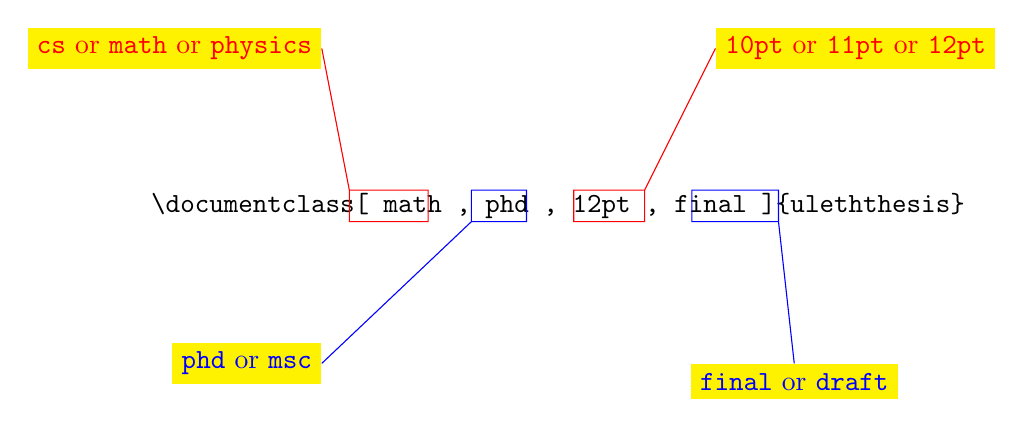
\begin{tikzpicture}
 \draw (0,0) node {\verb!\documentclass[ math , phd , 12pt , final ]{uleththesis}!};
 \draw[color=red]  (-1.65,-0.2) rectangle (-2.65,0.2) -- (-3,2) node[anchor=east,fill=yellow] {\verb!cs! or \verb!math! or \verb!physics!};
 \draw[color=blue] (-0.4,0.2) rectangle (-1.1,-0.2) -- (-3,-2) node[anchor=east,fill=yellow] {\verb!phd! or \verb!msc!};
 \draw[color=red]  (0.2,-0.2) rectangle (1.1,0.2) -- (2,2) node[anchor=west,fill=yellow] {\verb!10pt! or \verb!11pt! or \verb!12pt!};
 \draw[color=blue] (1.7,0.2) rectangle (2.8,-0.2) -- (3,-2) node[anchor=north,fill=yellow] {\verb!final! or \verb!draft!};
\end{tikzpicture}

\item Fill in the following information:
\texttt{\textbackslash title},
\texttt{\textbackslash author},
\texttt{\textbackslash degreeyear},
\texttt{\textbackslash prevdegrees}.


\item Add a signature line for every committee member, supervisor and thesis chair using \texttt{\textbackslash addsignatureline}.

\item Write your dedication inside the \texttt{\textbackslash dedication\{\}} section.

\item Write your abstract inside the \texttt{\textbackslash begin\{abstract\}} ~~~ \texttt{\textbackslash end\{abstract\}}.

\item Write you acknowledgments inside the \texttt{\textbackslash acknowledgments\{\}} section.

\item  ~ \\
\begin{tikzpicture}
 \draw (0,0) node[anchor=west] {\verb!\chapter[Introduction]{Introduction}
\chaptermark{Introduction}
\label{ch:introduction}

\hfill\begin{tabular}{r}\toprule
 {\it `Obvious' is the most dangerous} \\ {\it word in mathematics.} \\
  -- E. T. Bell\\
\bottomrule\end{tabular}\vskip25pt

This thesis is a combination of many novel ideas that have been studied in the past few years. The bulk of the study has been centred around the idea of biangular line-sets where we impose certain conditions in order to obtain specific combinatorial objects. The work found within is a combination of published work,~\cite{much10,unit-weigh13}, submitted work,~\cite{muwm13}, and forthcoming publications.

Hadamard matrices have garnered the interest of many mathematicians and physicists over the past century. With their impeccable structure, it is no surprise that these objects appear in many seemingly unrelated areas (see~\cite{hada-app2,hada-app,space-time-block}). At their historical roots, Hadamard matrices were studied by James Sylvester in 1867, who focused on a specialized infinite family of Hadamard matrices~\cite{sylvester}.

Nearly 25 years later, Jacques Hadamard constructed the first two Hadamard matrices that did not fit into Sylvester's specialized case~\cite{hadamard}. Furthermore, Hadamard gave an infinite family of his own. Soon after, a very famous conjecture was formuated: that there is a Hadamard matrix for every order that is a multiple of 4. This hypothesis has come to be known as the {\it Hadamard conjecture}.

It is now more than a century later, and many more examples of Hadamard matrices have been found. There have been many steps towards a resolution of the Hadamard conjecture. However, while we are edging towards a resolution of this conjecture, we are still lacking the key insight that is needed to finally put a pin in it.

Many generalizations of Hadamard matrices have emerged over the years: orthogonal designs, weighing matrices~\cite{od-quad-forms} and unit Hadamard matrices~\cite{Dita_2004} to name a few. In this thesis, we introduce another extension of Hadamard matrices, unit weighing matrices, and classify them for many small orders and weights. These matrices give us most of the structure that is held by Hadamard matrices, as well as the extra flexibility needed to solve certain problems.

We then utilize these matrices by introducing yet another topic: mutually unbiased weighing matrices. These are an extension of the well-known mutually unbiased bases~\cite{durt-muhm}. Once again, we lose a little structure by dealing with weighing matrices instead of Hadamard matrices, but this loss of rigidity allows us to solve some problems that cannot be done with Hadamard matrices.
% We also pose a modified definition for mutually unbiased Hadamard matrices to allow for the inclusion of a new class of unbiasedness.

Majority of the content in the thesis will be used directly or indirectly to solve problems related to sets of vectors which have {\it nice} pairwise inner products. To be more specific, the inner product of any two vectors in the set must have a particular absolute value. There is a well-known upper bound on the size of these sets~\cite{calderbank97}, which we use as the ground work for our searches. In many small cases, the upper bound can be obtained by vectors which are taken directly from the objects created in the first few chapters.

In the final chapter, we use these {\it nice} sets to generate combinatorial objects. Many of these objects were previously unknown. For the objects which were already known, the methods to provide them are novel.

We will split our time in this thesis between the real and the complex case. The reader is urged to keep this in mind as they progress through this thesis, since many theorems come in two forms: the real case and the complex case. When it is not specified, it is assumed that the theorem is true in the complex case (and thus, the real case as well).

\section[A Note on Notation]{A Note on Notation}
\sectionmark{Notation}
\label{sec:notation}

Mathematicians are notorious for generating acronyms for subject matter. In this thesis, we will refrain from utilizing these acronyms as most of them will look too similar and are likely to cause headaches (e.g., MUBs, MUHM, MUCH, MUH, MOLS, MSLS, MUWM, MUCWM, MUUWM, etc.). With that being said, when these objects are introduced, we will specify the acronym for any reader who wishes to read other articles within the field where these acronyms are used heavily.

Any variable which utilizes a capital letter is a matrix. $I_n$ is the identity matrix of order $n$ and $J_n$ is the square all-ones matrix of order $n$. For $I_n$, the $n$ will be dropped when it can be inferred from context. You may also assume, without fault, that any $H$ or $W$ in this thesis represents a Hadamard matrix or a weighing matrix, respectively. For any matrix $X$, its transpose, entry-wise conjugation and Hermitian transpose are denoted by $X^T$, $\overline{X}$ and $X^*$, respectively. When matrices are explicitly written, any blank entries are zeroes. The indices of matrices will be 0-based.

The set of unimodular numbers, i.e., complex numbers with an absolute value of 1, will be denoted $\T$. Furthermore, $\T_0$ will be used to denote $\T \cup \left\{0\right\}$.

When a ``$-1$'' is to appear in a matrix, the shortened ``$-$'' within the matrix will be used. For example, instead of writing
$$H=\left(\begin{array}{rr}1&1 \\ 1&-1\end{array}\right),$$
we will instead use
$$H=\left(\begin{array}{cc}\Zp\Zp \\ \Zp\Zm\end{array}\right).$$

We would also like to warn the reader that $\omega$ is used in this thesis to mean different values at different portions of the thesis. You may assume, however, that it will represent some root of unity.

Finally, we would also like to point out that Jacques Hadamard was a French mathematician, meaning that the `H' at the beginning of his last name is silent. However, for this thesis, we will use the anglicized version of his name by saying `{\it a Hadamard matrix}' in lieu of the correct `{\it an Hadamard matrix}'.
!};
 \draw (0,-0.5) node[anchor=west] {\verb!\chapter[Background]{Background}
\sectionmark{Background}
\label{ch:background}

\hfill\begin{tabular}{r}\toprule
 {\it The shortest path between two truths} \\ {\it in the real domain passes} \\ {\it through the complex domain.} \\
  -- J. Hadamard\\
\bottomrule\end{tabular}\vskip25pt

We begin our campaign by giving a definition, which will lay the foundation for the entire thesis.

\begin{definition} \label{def:hadamard}
 A {\it real Hadamard matrix} (usually referred to as just a {\it Hadamard matrix} or shortened to be an $H$-matrix) is an $n \times n$ matrix consisting of entries in $\left\{ \pm 1 \right\}$ such that $HH^T = nI_n$.
\end{definition}

\begin{example} \label{ex:hadamard}

Here are three Hadamard matrices of orders 2, 4 and 8.

 $$H_2 = \left(\begin{array}{c}
               \Zp\Zp \\
               \Zp\Zm
              \end{array}\right), ~
  H_4 = \left(\begin{array}{c}
               \Zp\Zp\Zp\Zm \\
               \Zp\Zp\Zm\Zp \\
               \Zp\Zm\Zp\Zp \\
               \Zm\Zp\Zp\Zp
              \end{array}\right) \text{ and }$$

$$H_8 = \left(\begin{array}{c}
               \Zp\Zp\Zp\Zm\Zm\Zm\Zm\Zp \\
               \Zp\Zp\Zp\Zm\Zp\Zp\Zp\Zm \\
               \Zp\Zp\Zm\Zp\Zp\Zp\Zm\Zp \\
               \Zp\Zm\Zp\Zp\Zp\Zm\Zp\Zp \\
               \Zp\Zp\Zm\Zp\Zm\Zm\Zp\Zm \\
               \Zm\Zp\Zp\Zp\Zp\Zm\Zm\Zm \\
               \Zm\Zp\Zp\Zp\Zm\Zp\Zp\Zp \\
               \Zp\Zm\Zp\Zp\Zm\Zp\Zm\Zm \\
              \end{array}\right).$$

\end{example}

For the sake of this thesis, it is important to notice that we can view the rows of a Hadamard matrix as a collection of $n$ vectors in $\left\{\pm1\right\}^n$ that are pairwise orthogonal. This idea of deconstructing matrices into vectors will be revisited throughout the thesis.

\section[Equivalence of Hadamard Matrices]{Equivalence of Hadamard Matrices}
\sectionmark{Equivalence of Hadamard Matrices}
\label{sec:equiv}

At first glance, the locations of the positives and negatives in a Hadamard matrix seem quite random. We will soon see that we may alter the way that these matrices look to give us a better sense of the underlying structure of the matrices.

\begin{proposition} \label{prop:equiv-hadamard}
 If $H$ is a Hadamard matrix, then so are $H^T$ and $PHQ$, where $P$ and $Q$ are signed-permutation matrices.
 \begin{proof}
  We will prove both claims directly from the definition of Hadamard matrices. By the definition of a Hadamard matrix, we have that $H^{-1} = \frac{1}{n}H^T$. This implies $$H^T\left(H^T\right)^T = nH^{-1}H = nI.$$ Secondly, $\left(PHQ\right)\left(PHQ\right)^T = PHQQ^TH^TP^T = nI$ since $P$ and $Q$ are orthogonal matrices.
 \end{proof}
\end{proposition}

With this in our pocket, we will introduce the following.

\begin{definition} \label{def:equiv-hadamard}
 Two Hadamard matrices, $H_1$ and $H_2$, are said to be {\it equivalent} if there exist two signed-permutation matrices, say $P$ and $Q$, such that $H_1 = PH_2Q$. Equivalence is denoted by $H_1 \cong H_2$.
\end{definition}
In a more direct sense, this means that we may permute or negate the rows and the columns of our matrix without affecting which equivalence class the matrix is in. It is important to note that the transpose of $H$ is not included in Definition~\ref{def:equiv-hadamard}; some authors do include $H^T$ as part of the equivalence, but we do not.

\begin{definition} \label{def:dephased}
 A Hadamard matrix is {\it dephased} if the first row and first column contain only ones.
\end{definition}

Which immediately leads us to the following.

\begin{lemma} \label{lem:dephased}
 Every Hadamard matrix is equivalent to a dephased Hadamard matrix.
 \begin{proof}
  For each column, look at the first entry. If it is $-1$, then negate that column. Then repeat the process for the rows. The resulting equivalent matrix will be dephased.
 \end{proof}

\end{lemma}

Determining the number of inequivalent Hadamard matrices is a very laborious task. The classification of Hadamard matrices has been an ongoing process over the past few decades. In the next section, we will see that Hadamard matrices can only exist if $n \leq 2$ or $n$ is a multiple of 4. A very simple program can be written to determine the number of inequivalent Hadamard matrices of order $n \leq 24$. For $n = 28$, decades were needed to fully classify all 487 Hadamard matrices of order $28$~\cite{classification28}. In 2013, Kharaghani and Tayfeh-Rezaie finished the classification of Hadamard matrices of order 32~\cite{hada32}. The number of inequivalent Hadamard matrices can be found in Table~\ref{table:inequiv-hada}.

\begin{table}[ht]
\caption{Number of inequivalent Hadamard matrices of order $n$ ($n \leq 32$)}
\label{table:inequiv-hada}
\centering
\begin{tabular}{@{}lcr@{}}
\hline
\toprule
\multicolumn{1}{@{}c@{}}{$n$} && \multicolumn{1}{@{}c@{}}{\# Matrices}\\
\midrule
 1  && 1 \\
 2  && 1 \\
 4  && 1 \\
 8  && 1 \\
 12 && 1 \\
 16 && 5 \\
 20 && 3 \\
 24 && 60 \\
 28 && 487 \\
 32 && 13710027 \\
\bottomrule
 \end{tabular}
\end{table}

\section[Existence of Hadamard Matrices]{Existence of Hadamard Matrices}
\sectionmark{Existence of Hadamard Matrices}
\label{sec:existence}

A few observations can be made about Hadamard matrices. It is immediate to note that the order of a Hadamard matrix must be even, but it takes a little closer inspection to note that the order must be small or a multiple of four.

\begin{lemma} \label{lem:mult-4}
 If $n > 2$ is the order of a Hadamard matrix, then $n$ is a multiple of four.
 \begin{proof}
  Let $H$ be a Hadamard matrix of order $n > 2$. By Lemma~\ref{lem:dephased}, we know that $H$ is equivalent to a dephased Hadamard matrix, say $H'$. Let's examine the first three rows of $H'$. We may permute the columns of this submatrix in such a way that we arrive at the following

 \begin{center}
 \begin{tikzpicture}[decoration=brace]
    \matrix (m) [matrix of math nodes,left delimiter=(,right delimiter={)}] {
        \Zp\Zp\cdots\Zp\Zp & \Zp\Zp\cdots\Zp\Zp & \Zp\Zp\cdots\Zp\Zp & \Zp\Zp\cdots\Zp\Zp \\
        \Zp\Zp\cdots\Zp\Zp & \Zp\Zp\cdots\Zp\Zp & \Zm\Zm\cdots\Zm\Zm & \Zm\Zm\cdots\Zm\Zm \\
        \Zp\Zp\cdots\Zp\Zp & \Zm\Zm\cdots\Zm\Zm & \Zp\Zp\cdots\Zp\Zp & \Zm\Zm\cdots\Zm\Zm \\
        \vdots & \vdots & \vdots & \vdots \\
    };
    \draw[decorate,transform canvas={yshift=0.5em},thick] (m-1-1.north west) -- node[above=2pt] {$a$ columns} (m-1-1.north east);
    \draw[decorate,transform canvas={yshift=0.5em},thick] (m-1-2.north west) -- node[above=2pt] {$b$ columns} (m-1-2.north east);
    \draw[decorate,transform canvas={yshift=0.5em},thick] (m-1-3.north west) -- node[above=2pt] {$c$ columns} (m-1-3.north east);
    \draw[decorate,transform canvas={yshift=0.5em},thick] (m-1-4.north west) -- node[above=2pt] {$d$ columns} (m-1-4.north east);
\end{tikzpicture}.
 \end{center}

\noindent That is, we permute the columns in such a way that the the first $a$ columns have exactly three ones in the first three rows, the next $b$ columns have a one in the first two rows and a $-1$ in the third row, the next $c$ columns' first three rows are $1, -1, 1$, respectively and the last $d$ columns have $1, -1, -1$ in their first three rows.
  
   From the orthogonality of each of the three pairs of rows, as well as imposing that the order of the matrix is $n$, we have
$$\begin{cases}
  a + b + c + d = n \\
  a + b - c - d = 0 \\
  a - b + c - d = 0 \\
  a - b - c + d = 0
 \end{cases}$$
 which has the unique solution of $a = b = c = d = n/4$. Since $a, b, c, d$ and $n$ are all integers, we have that $n$ must be a multiple of 4.
 \end{proof}
\end{lemma}

It is a common belief that this is the only obstacle that must be overcome. In fact, we have the following famous conjecture.

\begin{conjecture}[Hadamard Conjecture] \label{conj:hadamard-conjecture}
 If $n = 4k$ for some $k \geq 1$, then there exists a Hadamard matrix of order $n$.
\end{conjecture}

Prior to 2004, Conjecture~\ref{conj:hadamard-conjecture} had been verified for all $n < 428$. In 2004, Kharaghani and Tayfeh-Rezaie found a Hadamard matrix of order 428~\cite{hada428}, leaving $n = 668$ as the smallest order for with the Hadamard conjecture has not been verified.

\section[Construction of Hadamard Matrices]{Construction of Hadamard Matrices}
\sectionmark{Construction of Hadamard Matrices}
\label{sec:construction}

The study of Hadamard matrices started nearly a century and a half ago when James Sylvester constructed an infinite family of matrices which satisfied the condition laid out in Definition~\ref{def:hadamard} (even though they were not called ``Hadamard matrices'' at the time).

\begin{theorem}[Sylvester,~\cite{sylvester}] \label{th:syl}
 If $H$ is a Hadamard matrix, then $$\left(\begin{array}{cc}H&H\\H&-H\end{array}\right)$$ is also a Hadamard matrix.
 \begin{proof}
  This can easily be verified straight from the definition.
 \end{proof}
\end{theorem}

The observation in Theorem~\ref{th:syl} was crucial to the generation of the following infinite class of Hadamard matrices which are today called {\it Sylvester matrices}.

\begin{corollary}[Sylvester,~\cite{sylvester}] \label{cor:syl}
 There exists a Hadamard matrix of order $2^k$ for any $k \geq 0$.
 \begin{proof}
  $H=\left(\begin{array}{c}1\end{array}\right)$ is a Hadamard matrix. Apply Theorem~\ref{th:syl} $k$ times to $H$.
 \end{proof}
\end{corollary}

Jacques Hadamard was the next mathematician to examine these matrices in detail. He was looking for examples of matrices whose determinants attained the following upper bound.

\begin{theorem}[Hadamard,~\cite{hadamard}] \label{th:hada-bound}
 If $\{v_{0},\dots,v_{n-1}\}$ are the rows of a square matrix $A$, then \begin{equation}\label{eq:hadamard-bound-a}|\det(A)| \leq \displaystyle\prod_{i=0}^{n-1}||v_i||.\end{equation} Moreover, if every entry's absolute value is at most $B \in \R$, then \begin{equation}\label{eq:hadamard-bound-b}|\det(A)| \leq B^nn^{n/2}.\end{equation}
\end{theorem}

It is natural to study the case where $B=1$ in Theorem~\ref{th:hada-bound} since all matrices may be scaled to this value. With this appropriate scaling, Hadamard showed that the bound (\ref{eq:hadamard-bound-b}) is realized in the real case if and only if $A$ is a Hadamard matrix~\cite{hadamard}. In the same article, Hadamard constructed Hadamard matrices of order 12 and 20. These are the smallest order that do not fit into Sylvester's infinite class. Hadamard also gave a more generalized version of Sylvester's construction which can most easily be described through use of the Kronecker product.

\begin{definition} \label{def:kronecker-product}
 Let $A = [a_{ij}]$ and $B = [b_{ij}]$ be $m \times n$ and $p \times q$ matrices, respectively. The {\it Kronecker product} of $A$ and $B$, denoted $A \otimes B$, is the following $mp \times nq$ matrix

 $$\left(\begin{array}{ccccc}
          a_{0,0}B & \cdots  & a_{0,n-1}B \\
           \vdots & \ddots & \vdots \\
          a_{m-1,1}B & \cdots  & a_{m-1,n-1}B
         \end{array}\right).$$
\end{definition}

The following is an immediate way to construct new Hadamard matrices from old ones.

\begin{lemma}[Hadamard,~\cite{hadamard}] \label{lem:kronecker}
 If $H_1$ and $H_2$ are Hadamard matrices of order $m$ and $n$, respectively, then $H_1 \otimes H_2$ is a Hadamard matrix of order $mn$.
 \begin{proof}
  $$(H_1 \otimes H_2)(H_1 \otimes H_2)^T = H_1H_1^T \otimes H_2H_2^T = mI_m \otimes nI_n = mnI_{mn}$$
 \end{proof}
\end{lemma}

This new construction method means that when any new Hadamard matrix is formed, we may use the Kronecker product to give us many (possibly new) Hadamard matrices. But unfortunately, this construction comes with an inherent problem. Creating Hadamard matrices of order $4n$ where $n$ is even is quite a bit easier than when $n$ is odd. With the method above, Hadamard matrices of order $4a$ and $4b$ will be able to construct a new Hadamard matrix of order $16ab$. The following construction allows us to create a Hadamard matrix of half of that order.

% Need to \CITE
\begin{theorem}[\mbox{\cite{8ab}}] \label{thm:8ab-construction}
 If there exist Hadamard matrices of order $4a$ and $4b$, then there exists a Hadamard matrix of order $8ab$.
 \begin{proof}
  Let $H_1$ be a Hadamard matrix of order $4a$ and $H_2$ be a Hadamard matrix of order $4b$. Let $A$ and $B$ be $4a \times 2a$ matrices and let $C$ and $D$ be $2b \times 4b$ matrices such that
$$ H_1 = \left(\begin{array}{cc}A&0\end{array}\right) + \left(\begin{array}{cc}0&B\end{array}\right) \text{ and } H_2 = \left(\begin{array}{c}C \\ 0\end{array}\right) + \left(\begin{array}{c}0 \\ D\end{array}\right).$$
We then form
$$H = \frac12\left(A + B\right) \otimes C + \frac12\left(A-B\right) \otimes D.$$

It is important to note that if we examine corresponding entries in $A+B$ and $A-B$, then exactly one of them is zero and the other is either $2$ or $-2$. Thus, each entry in $H$ is either $1$ or $-1$. Next, let us examine the following product.

\equationarray
$$\begin{array}{rcl}
HH^T &=& \left(\frac12\left(A + B\right) \otimes C + \frac12\left(A-B\right) \otimes D\right)\left(\frac12\left(A + B\right) \otimes C + \frac12\left(A-B\right) \otimes D\right)^T \\
 &=&
\left(\frac12\left(A + B\right) \otimes C\right)\left(\frac12\left(A + B\right) \otimes C\right)^T +
\left(\frac12\left(A-B\right) \otimes D\right)\left(\frac12\left(A-B\right) \otimes D\right)^T \\
 & & +
\left(\frac12\left(A + B\right) \otimes C\right)\left(\frac12\left(A-B\right) \otimes D\right)^T +
\left(\frac12\left(A-B\right) \otimes D\right)\left(\frac12\left(A + B\right) \otimes C\right)^T \\
 &=&
\left(\frac14\left(A + B\right)\left(A + B\right)^T\right) \otimes CC^T +
\left(\frac14\left(A - B\right)\left(A - B\right)^T\right) \otimes DD^T \\
 & & +
\left(\frac14\left(A + B\right)\left(A - B\right)^T\right) \otimes CD^T +
\left(\frac14\left(A - B\right)\left(A + B\right)^T\right) \otimes DC^T \\

 &=&
\left(\frac14\left(A + B\right)\left(A + B\right)^T\right) \otimes 4bI_{2b} +
\left(\frac14\left(A - B\right)\left(A - B\right)^T\right) \otimes 4bI_{2b} \\
 & & +
\left(\frac14\left(A + B\right)\left(A - B\right)^T\right) \otimes 0_{2b} +
\left(\frac14\left(A - B\right)\left(A + B\right)^T\right) \otimes 0_{2b} \\
 &=& 
\left[\left(\frac14\left(A + B\right)\left(A + B\right)^T\right) +
\left(\frac14\left(A - B\right)\left(A - B\right)^T\right)\right] \otimes 4bI_{2b}\\
 &=&
\left[\frac12 \left(AA^T + BB^T\right)\right] \otimes 4bI_{2b} \\
 &=&
\frac12 \left(4a I_{4a} \right) \otimes 4bI_{2b} \\
 &=&8abI_{8ab}
\end{array}$$
\normalarray
which implies, from Definition~\ref{def:hadamard}, that $H$ is a Hadamard matrix.
 \end{proof}
\end{theorem}

The first infinite class of Hadamard matrices of order $4n$ which includes many values for which $n$ is odd is attributed to Paley. Before stating the result, we must first take a small detour through some field theory results.

\begin{definition} \label{def:field-stuff}
 Let $\F_p$ be a finite field of order $p$ and let $a$ be a nonzero element of $\F_p$. $a$ is a {\it quadratic residue mod $p$} if there exists $b \in \F_p$ such that $a \equiv b^2 \pmod p$. The {\it Legendre symbol mod} $p$, $\chi: \F_p \rightarrow \Z$, is defined as

 $$\chi(a) = \begin{cases}
             0 & \text{if } a = 0, \\
             1 & \text{if } a \text{ is a quadratic residue mod } p, \\
             -1 & \text{otherwise.} \\
            \end{cases}$$

\end{definition}

\begin{lemma} \label{lem:half-quad}
 If $p$ is an odd prime number, then exactly $(p-1)/2$ elements in $\F_p$ are quadratic residues.

 \begin{proof}
  First, we note that for all $c \in \F_p$, $c^2 = (-c)^2$, so there are at most $(p-1)/2$ quadratic residues. To avoid these trivial collisions, we will examine $a,b \in \F_p$ such that $1 \leq a, b \leq (p-1)/2$. If we also assume that $a^2 = b^2$, then we have $$(a+b)(a-b) = a^2 - b^2 = 0.$$ Since we are in a field, either $a+b = 0$ or $a-b = 0$. The first equality cannot hold since $a+b \in \left\{2,3,\dots,p-1\right\}$. The second equality is true if and only if $a = b$. So for any pair $(a,b)$ such that $1 \leq a \neq b \leq (p-1)/{2}$, we have that $a^2 \neq b^2$. Thus, there are at least $(p-1)/{2}$ quadratic residues mod $p$, and the result follows.
 \end{proof}

\end{lemma}

\begin{definition} \label{def:jacobsthal}
 Let $p$ be an odd prime number. Then we define the {\it Jacobsthal matrix} to be the $p \times p$ matrix, $Q_p = [q_{ij}]$, such that $$q_{ij} = \chi(i-j),$$ where $i-j$ is reduced mod $p$.
\end{definition}

\begin{theorem} \label{th:qqt}
 Let $p$ be an odd prime number. Then $Q_pQ_p^T = pI - J$.
 \begin{proof}
  Let $v_i$ and $v_j$ be the $i^{th}$ and $j^{th}$ rows of $Q_p$. If $i = j$, then $\langle v_i,v_j\rangle = p-1$ since there are exactly $p-1$ nonzeroes per row (each of which is $\pm 1$). Now, assume that $i \neq j$, then we have that

  $$\langle v_i,v_j \rangle = \sum_{a \in \F_p} \chi(i-a)\chi(j-a) = \sum_{b \in \F_p} \chi(b)\chi(b+(j-i)).$$ From here, we note that when $b=0$, $\chi(b) = 0$, so we have $$\langle v_i,v_j \rangle = \sum_{b \in \F_p \setminus \{0\}} \chi(b)\chi(b+(j-i)).$$
  Next, we will use the fact that $\chi$ is a multiplicative function to see that 
  $$\langle v_i,v_j \rangle = \sum_{b \in \F_p \setminus \{0\}} \chi(b)\chi(b)\chi(1+b^{-1}(j-i)) = \sum_{b \in \F_p \setminus \{0\}} \chi(1+b^{-1}(j-i))$$
  Since $j-i$ is fixed and nonzero, $1+b^{-1}(j-i)$ will run through each element in $\F_p$ except $1$. By using Lemma~\ref{lem:half-quad} and the fact that $\chi(1) = 1$ for all $p$,
  $$\langle v_i,v_j \rangle = \sum_{c \in \F_p \setminus \{1\}} \chi(c) = \left(\sum_{c \in \F_p} \chi(c)\right) - \chi(1) = 0 - 1 = -1.$$
  Thus, the inner product of two distinct rows of $Q_p$ are $-1$, and the result follows.
 \end{proof}

\end{theorem}


\begin{theorem}[Paley,~\cite{paley}] \label{thm:paley-3}
 Let $p \equiv 3\pmod4$ be an odd prime number. Then
  $$H = \left(\begin{array}{cc}
     1 & 1_{p} \\
     1_{p}^T & Q_p-I
    \end{array}\right)$$
  is a Hadamard matrix of order $p+1$, where $1_p$ is a row vector of $p$ ones.

 \begin{proof}
  \equationarray
  $$\begin{array}{rcll}
     HH^T &=& \left(\begin{array}{cc}
     1 & 1_{p} \\
     1_{p}^T & Q_p-I
    \end{array}\right)
    \left(\begin{array}{cc}
     1 & 1_{p} \\
     1_{p}^T & Q_p-I
    \end{array}\right)^T \\
  & = &
    \left(\begin{array}{cc}
     p+1 & 0_p \\
     0_p^T & J + (Q_p-I)(Q_p-I)^T
     \end{array}\right)\\
  & = &
    \left(\begin{array}{cc}
     p+1 & 0_p \\
     0_p^T & J + Q_pQ_p^T-Q_p-Q_p^T+I
     \end{array}\right)\\
  & = &
    \left(\begin{array}{cc}
     p+1 & 0_p \\
     0_p^T & J + Q_pQ_p^T+I
     \end{array}\right) & \left(\text{since } Q_p = -Q_p^T \text{ if } p\equiv 3\hskip-10pt\pmod4\right)\\
  & = &
    \left(\begin{array}{cc}
     p+1 & 0_p \\
     0_p^T & J + (pI-J)+I
     \end{array}\right) & \left(\text{by Theorem~\ref{th:qqt}}\right)\\
  & = &
    \left(\begin{array}{cc}
     p+1 & 0_p \\
     0_p^T & (p+1)I_{p}
     \end{array}\right)\\
  & = & (p+1)I_{p+1}
    \end{array}$$ %End of equation array.
  \normalarray
 \end{proof}

\end{theorem}

\begin{theorem}[Paley,~\cite{paley}] \label{thm:paley-1}
 Let $p \equiv 1 \pmod 4$ be an odd prime number. Then
  $$H = \left(\begin{array}{cc|cc}
     1 & 1_{p}     & -1 & 1_{p}\\
     1_{p}^T & Q_p+I & 1_{p}^T & Q_p-I \\
     \hline
     -1 & 1_{p}     & -1 & -1_{p}\\
     1_{p}^T & Q_p-I & -1_{p}^T & -Q_p-I \\
    \end{array}\right)$$
  is a Hadamard matrix of order $2(p+1)$, where $1_p$ is a row vector of $p$ ones.

  \begin{proof}
  \equationarray
  $$\begin{array}{rcll}
     HH^T &=& \left(\begin{array}{cc|cc}
     1 & 1_{p}     & -1 & 1_{p}\\
     1_{p}^T & Q_p+I & 1_{p}^T & Q_p-I \\
     \hline
     -1 & 1_{p}     & -1 & -1_{p}\\
     1_{p}^T & Q_p-I & -1_{p}^T & -Q_p-I \\
    \end{array}\right)
    \left(\begin{array}{cc|cc}
     1 & 1_{p}     & -1 & 1_{p}\\
     1_{p}^T & Q_p+I & 1_{p}^T & Q_p-I \\
     \hline
     -1 & 1_{p}     & -1 & -1_{p}\\
     1_{p}^T & Q_p-I & -1_{p}^T & -Q_p-I \\
    \end{array}\right)^T \\
   & = &
    \left(\begin{array}{cccc}
     2(p+1) & 0 & 0 & 0\\
     0 & 2(J + Q_pQ_p^T + I) & 0 & 2(Q_p^T-Q_p) \\
     0 & 0 & 2(p+1) & 0 \\
     0 & 2(Q_p-Q_p^T) & 0 & 2(J + Q_pQ_p^T + I) \\
    \end{array}\right) \\
   & = &
    \left(\begin{array}{cccc}
     2(p+1) & 0 & 0 & 0\\
     0 & 2(J + (pI-J) + I) & 0 & 0 \\
     0 & 0 & 2(p+1) & 0 \\
     0 & 0 & 0 & 2(J + (pI-J) + I) \\
    \end{array}\right)\\
   & = &
    \left(\begin{array}{cccc}
     2(p+1) & 0 & 0 & 0\\
     0 & 2(p+1)I & 0 & 0 \\
     0 & 0 & 2(p+1) & 0 \\
     0 & 0 & 0 & 2(p+1)I \\
    \end{array}\right)\\
   & = & 2(p+1)I_{2(p+1)},
    \end{array}$$ %End of equation array.
   \normalarray
 where the third last equality is true since $Q_p = Q_p^T$ when $p \equiv 1 \pmod 4$.
 \end{proof}
\end{theorem}

Later, a similar idea was used to show that $p$ can be any odd prime power in the previous two lemmas through the use of finite fields. In 1944, Williamson introduced a new class of Hadamard matrices which needs the idea of circulant matrices.

\begin{definition} \label{def:circ-matrix}
 Given a vector of $n$ elements, $(v_0,v_1,\dots,v_{n-1})$,  a {\it circulant matrix}, $A = [a_{ij}]$, is a matrix defined as $a_{ij} = v_{i-j}$ where $i-j$ is reduced modulo $n$. Circulant matrices can be represented by their first row by $A = \text{Circ}(v_0,\dots,v_{n-1})$.
\end{definition}

From these, Williamson gave the following.

\begin{theorem}[\mbox{\cite{od-quad-forms}}]\label{thm:williamson}
 Let $A$, $B$, $C$ and $D$ be four symmetric circulant matrices of order $n$ which satisfy $$A^2 + B^2 + C^2 + D^2 = 4nI_n.$$ Then
$$\left(\begin{array}{rrrr}
         A & B & C & D \\
         -B & A & -D & C \\
         -C & D & A & -B \\
         -D & -C & B & A
        \end{array}
\right)$$
is a Hadamard matrix of order $4n$.
 \begin{proof}
  This can easily be verified by multiplying out the matrix with its transpose and utilizing our assumption.
 \end{proof}

\end{theorem}

\begin{example}
 For example, $A = \text{Circ}(1~1~1)$, $B=C=D=\text{Circ}(-~1~1)$ satisfies the conditions laid out in Theorem~\ref{thm:williamson}, and so we may create a $12 \times 12$ Hadamard matrix.
\end{example}

These constructions account for a large portion of the Hadamard matrices that are currently known, especially for smaller values. There are many other constructions for Hadamard matrices, most of which are out of the scope of this thesis (see~\cite{od-quad-forms} for more constructions).!};
 \draw (0,-1) node[anchor=west] {\verb!\chapter[Generalizations of Hadamard Matrices]{Generalizations of Hadamard Matrices}
\chaptermark{Generalizations}
\label{ch:generalizations}

\hfill\begin{tabular}{r}\toprule
 {\it Curiosity.} \\ {\it Not good for cats,} \\ {\it but very good for scientists.} \\
 -- L. Fleinhardt\\
\bottomrule\end{tabular}\vskip25pt

(This chapter is based on published work, \cite{unit-weigh13}.)

In this chapter, we introduce the idea of unit weighing matrices. These matrices are a generalization of Hadamard matrices. We fully classify the matrices for small orders and then proceed to show their usefulness in Chapter~\ref{ch:unbiased}.

When Hadamard matrices were originally studied, they were square matrices with entries in $\{\pm1\}$ which contained mutually orthogonal rows (as defined in Definition~\ref{def:hadamard}). There have been quite a few generalizations of Hadamard matrices that have appeared over the years. We will examine two of these generalizations which have been explored extensively in the literature.

\section{Weighing Matrices}

First, we will remove the restriction that the entries must be in the set $\{\pm1\}$ by allowing a third entry, 0.

\begin{definition} \label{def:weigh}
 An $n \times n$ matrix, $W$, with entries in $\{0,\pm1\}$ such that $WW^T = wI$ for some $w$ is called a {\it weighing matrix} of order $n$ and weight $w$. Weighing matrices are often denoted $W(n,w)$.
\end{definition}

\begin{example} \label{ex:weigh}
$W_7$ is a weighing matrix of order 7 and weight 4, a $W(7,4)$.
$$W_7=\left(\begin{array}{ccccccc}
1 & 1 & 1 & 1 & 0 & 0 & 0 \\
1 & - & 0 & 0 & 1 & 1 & 0 \\
1 & 0 & - & 0 & - & 0 & 1 \\
1 & 0 & 0 & - & 0 & - & - \\
0 & 1 & - & 0 & 0 & 1 & - \\
0 & 1 & 0 & - & 1 & 0 & 1 \\
0 & 0 & 1 & - & - & 1 & 0
\end{array}\right)$$
\end{example}

We note that a $W(n,n)$ is a Hadamard matrix. Unlike Hadamard matrices, however, the order of weighing matrices are not restricted nearly as much. For example, the matrix given in Example \ref{ex:weigh} is of order 7, which is not a multiple of 4. We have the following extension of the Hadamard conjecture which states that a weighing matrix should exist for every weight of specific orders.

\begin{conjecture}[\cite{weighing-app}] \label{conj:weigh}
 Let $n$ be any integer multiple of four. Then there exists a weighing matrix of the type $W(n,w)$ for all $w \leq n$.
\end{conjecture}

% When the order of the matrix does not fall into the special case of being a multiple of four, there are restrictions that appear.

% \begin{theorem}[\cite{od-quad-forms}] \label{th:weigh-odd-n}
%  If $n \equiv 1 \pmod 2$ and a $W(n,w)$ exists, then $w$ is a perfect square. If $n \equiv 2 \pmod 4$, then $w$ must be the sum of two squares.
% \end{theorem}

We may define equivalence between weighing matrices in the same way that we define the equivalence of Hadamard matrices (i.e., row and column permutations and negations do not change which equivalence class you are in). Using this notion, Chan \etal classified all weighing matrices with weights smaller than 6 in 1986~\cite{inequiv-weigh}. However, while working on the matrices in the remaining portion of this section, we found a mistake in their classification of matrices of weight 5. Independently, Harada and Munemasa also discovered the error. We refer the reader to~\cite{Harada_Munemasa_2012} for the full details of where the matrices were missed. The classification of real weighing matrices of weights 1, 2, 3 and 4 will be dealt with in Subsection~\ref{subsec:w1}, Theorem~\ref{th:uw-n2}, Corollary~\ref{cor:w-n3-order} and Corollary~\ref{cor:w-4-count}, respectively. For this reason, we will jump right to the classification of weight 5 matrices and will deal with the first four later.

In order to classify these matrices, we must first introduce the direct sum.

\begin{definition} \label{def:direct-sum}
 Let $A$ and $B$ be two matrices of dimension $m \times n$ and $p \times q$, respectively. Then the {\it direct sum} of $A$ and $B$, denoted $A \oplus B$, is the $(m+p) \times (n+q)$ matrix $$\left(\begin{array}{cc}A&0\\0&B\end{array}\right).$$
\end{definition}


\begin{theorem}[\cite{inequiv-weigh,Harada_Munemasa_2012}] \label{th:class-wn5}
 Any $W(n,5)$ is equivalent to the direct sum of a specific set of weighing matrices. The set includes 5 sporadic cases and two infinite families.
\end{theorem}

The set of matrices that make up Theorem~\ref{th:class-wn5} (including the two that were originally missed) are in Appendix~\ref{app:real-wm}. Attempts have been made to classify weighing matrices for larger weights, but even in the next case, $w=6$, the complexity involved with the case analysis is immense. However, I feel that this classification could be completed within the next few years with a lot of elbow grease.

% \begin{problem} \label{prob:class-wn6}
%  Classify all weighing matrices of weight 6.
% \end{problem}

\subsection[Circulant Weighing Matrices]{Circulant Weighing Matrices}
\subsectionmark{Circulant Weighing Matrices}
\label{subsec:circ-weigh}

One very particular type of weighing matrices are those that are generated from circulating the first row.

\begin{definition} \label{def:circ-weigh}
 A {\it circulant weighing matrix} is a circulant matrix (see Definition~\ref{def:circ-matrix}) that is also a weighing matrix. In literature, circulant weighing matrices of order $n$ and weight $w$ are denoted by $CW(n,w)$.
\end{definition}

\begin{example} \label{ex:circ-weigh}
 Here are two examples of circulant weighing matrices. $H_4$ is the lone non-trivial example of a circulant Hadamard matrix, while $W_7$ is a $CW(7,4)$.

 $$H_4 = \text{Circ}(\Zm\Zp\Zp\Zp) = \left(\begin{array}{c}\Zm\Zp\Zp\Zp\\\Zp\Zm\Zp\Zp\\\Zp\Zp\Zm\Zp\\\Zp\Zp\Zp\Zm\\\end{array}\right)$$
 $$W_7 = \text{Circ}(\Zp\Zz\Zp\Zp\Zm\Zz\Zz) = \left(\begin{array}{c}
\Zp\Zz\Zp\Zp\Zm\Zz\Zz\\
\Zz\Zp\Zz\Zp\Zp\Zm\Zz\\
\Zz\Zz\Zp\Zz\Zp\Zp\Zm\\
\Zm\Zz\Zz\Zp\Zz\Zp\Zp\\
\Zp\Zm\Zz\Zz\Zp\Zz\Zp\\
\Zp\Zp\Zm\Zz\Zz\Zp\Zz\\
\Zz\Zp\Zp\Zm\Zz\Zz\Zp\\
\end{array}\right)$$

\end{example}


\begin{definition} \label{def:hall-poly}
 Given a circulant weighing matrix, $W = \text{Circ}(a_0,a_1,\dots,a_{n-1})$, the associated {\it Hall polynomial} is defined as $f(t) := \displaystyle\sum_{i=0}^{n-1}a_it^i$.
\end{definition}

\begin{lemma} \label{lem:hall-poly}
 Let $W$ be a circulant weighing matrix of order $n$ and weight $w$. If $f(t) = a_0 + \cdots a_{n-1}t^{n-1}$ is the associated Hall polynomial of $W$, then $f(\omega)f(\overline{\omega}) = w$ for all $n^{th}$ roots of unity, $\omega$.
 
 \begin{proof}
  $$f(\omega)f(\overline{\omega}) = (a_0 + a_1\omega + \cdots + a_{n-1}\omega^{n-1})(a_0 + a_1\overline{\omega} + \cdots + a_{n-1}\overline{\omega^{n-1}})$$
  $$=\sum_{d=0}^{n-1} \left(\omega^d \left[\sum_{i=0}^{n-1} a_ia_{i-d}\right]\right),$$ where the indices are being reduced mod $n$. In the sum above, the inner summation represents the inner products of two rows of $W$. Thus, we have that
  
  $$f(\omega)f(\overline{\omega})=w + \sum_{d=1}^{n-1}\left( \omega^d \left[0\right]\right) = w.$$
  
 \end{proof}

\end{lemma}

\begin{theorem} \label{th:circ-perf-sqr}
 Let $W$ be a circulant weighing matrix of order $n$ and weight $w$. Then $w$ must be a perfect square.

 \begin{proof}
  Let $W$ be a circulant weighing matrix and let $f(t)$ be the associated Hall polynomial. By Lemma~\ref{lem:hall-poly}, we have that $f(1)^2 = w$. Since $f(1)$ is simply the sum of the entries in any given row of $W$, it must be an integer, so $w$ is a perfect square.
 \end{proof}

\end{theorem}


A lot of interest has been shown in circulant weighing matrices, but most of the results are outside the scope of this thesis. For further details that are not provided here, we recommend~\cite{SchmidtSmith} and the references therein for general knowledge and~\cite {circ-weigh-9,circ-weigh-10,strassler-thesis,circ-prime} for the classification of small circulant weighing matrices.

\section[Unit Hadamard Matrices]{Unit Hadamard Matrices}
\sectionmark{Unit Hadamard Matrices}
\label{sec:unit-hada}

Another generalization of Hadamard matrices is to remove the restriction that the matrices must be real.

\begin{definition} \label{def:unit-hada}
 An $n \times n$ matrix, $H$, with all unimodular entries such that $HH^* = nI_n$ is called a {\it unit Hadamard matrix}.
\end{definition}

Other names for unit Hadamard matrices are {\it generalized Hadamard matrices} and {\it complex Hadamard matrices}\footnote{Be warned that the term ``complex Hadamard matrices'' has been used by different authors to mean different things.}.

Unit Hadamard matrices are the one and only type of matrix that we will discuss that have no restrictions on the order. In fact, we have the following strong theorem.

\begin{theorem} \label{th:fourier}
 There exists a unit Hadamard matrix for any order $n \geq 1$.
 \begin{proof}
  The proof is immediate by noting that the Fourier matrix of order $n$, $F = [f_{jk}]$, is a unit Hadamard matrix where $$f_{jk} = e^{jk\cdot2\pi i/n}$$ for all $0 \leq j, k < n$.
 \end{proof}

\end{theorem}

\begin{example} \label{ex:fourier}
 Here are the first three Fourier matrices, where $\omega = e^{2\pi i/3}$.
 $$\left(\begin{array}{c}1\end{array}\right) , \left(\begin{array}{cc}1&1\\1&-\end{array}\right) \text{ and } \left(\begin{array}{ccc}1&1&1\\1&\omega&\bar\omega\\1&\bar\omega&\omega\end{array}\right).$$
\end{example}

For a comprehensive look at unit Hadamard matrices, we refer the reader to Sz\"oll\H{o}si's Ph.D. thesis~\cite{ferenc-thesis}.

\section[Unit Weighing Matrices]{Unit Weighing Matrices}
\sectionmark{Unit Weighing Matrices}
\label{sec:unit-weigh}

In this thesis, we combine the previous two sections to introduce a new class of matrices.

\begin{definition} \label{def:unit-weigh}
 An $n \times n$ matrix, $W$, with entries in $\T_{0}$ such that $WW^*=wI_n$ for some $w$ is called a {\it unit weighing matrix}. Unit weighing matrices are denoted $UW(n,w)$.
\end{definition}

These matrices take a bit of weighing matrices and a bit of unit Hadamard matrices and fuse them together. By doing this, we open the door to solving many problems related to line-sets (these problems will be discussed further in Chapters~\ref{ch:unbiased} and~\ref{ch:app}).

In the rest of this chapter, we will start the classification process for unit weighing matrices. The classification of unit weighing matrices is much more difficult than the classification of real weighing matrices due to the fact that each entry of a unit weighing matrix has infinitely many choices.

\section[Equivalence of Unit Weighing Matrices]{Equivalence of Unit Weighing Matrices}
\sectionmark{Equivalence of Unit Weighing Matrices}
\label{sec:equiv-weigh}

The following proposition will serve as an analogue of Proposition~\ref{prop:equiv-hadamard}.

\begin{proposition} \label{prop:equiv-ops}
For a given unit weighing matrix, applying any of the following operations will result in a unit weighing matrix:
\begin{enumerate}
 \item[(T1)] Permuting the rows or columns.
 \item[(T2)] Multiplying any row or column of the matrix by a number in  $\mathbb{T}$.
 \item[(T3)] Taking the Hermitian transpose.
 \item[(T4)] Conjugating every entry in the matrix.
\end{enumerate}

\begin{proof}
 Each of these can be easily verified.
\end{proof}

\end{proposition}

Note that by applying $(T3)$ followed by $(T4)$, we have that the transpose of a unit weighing matrix is also a unit weighing matrix. From Proposition~\ref{prop:equiv-ops}, we may give a definition of equivalence similar to that of Definition~\ref{def:equiv-hadamard}.

\begin{definition} \label{def:equiv-weigh}
 Two unit weighing matrices, $W_1$ and $W_2$, are {\it equivalent} if one can be obtained from the other 
by performing a finite number of  operations $(T1)$ and $(T2)$ to it.
\end{definition}

Though Definitions~\ref{def:equiv-hadamard} and~\ref{def:equiv-weigh} are stated differently, they are essentially the same if one introduces the notion of a {\it unimodular permutation matrix}. Note that $(T3)$ and $(T4)$ are excluded from the definition in order to maintain consistency between the definitions of equivalence for Hadamard matrices and unit weighing matrices.

The first large difference between real weighing matrices and unit weighing matrices is the number of equivalence classes of matrices. In the real case, there are clearly only a finite number of classes. However, when we are dealing with unit weighing matrices, there may be infinitely many . In fact, there may be uncountably many, as we will see in the Example~\ref{ex:uw-44}. But first, we must introduce the following definition.

\begin{definition}[Haagerup's Invariant] \label{def:haargerup-inv}
 Let $W = [w_{ij}]$ be a unit weighing matrix. We define the following multiset\footnote{When we refer to multisets, we will represent them as a set of ordered pairs of the form ``(value,count)''. For example, $\{1,1,2,3,4,4,4\}$ would be represented as $\{(1,2),(2,1),(3,1),(4,3)\}$.}
$$\Lambda(W) = \left\{w_{ij}\overline{w_{kj}}w_{kl}\overline{w_{il}} :0 \leq i,j,k,l < n\right\}.$$
\end{definition}

With this, we can give the following strong theorem.

\begin{theorem} \label{th:equiv-haargerup}
 If two unit weighing matrices, $W_1$ and $W_2$, are equivalent, then $\Lambda(W_1) = \Lambda(W_2)$.
 \begin{proof}
  We note that the four operations in Proposition~\ref{prop:equiv-ops} do not affect this multiset, and so the result follows.
 \end{proof}

\end{theorem}

It is the contrapositive of this statement that is typically used. This has been used quite heavily to determine the inequivalence of unit Hadamard matrices. By using Theorem~\ref{th:equiv-haargerup}, we can see that there can be infinitely many inequivalent unit weighing matrices.

\begin{example} \label{ex:uw-44}
 There are infinitely many $UW(4,4)$.

 \begin{proof}
  Let $$W_4(x) = \left(\begin{array}{rrrr}1&1&1&1\\1&-&1&-\\1&1&x&-x\\1&-&-x&x\end{array}\right),$$ which is a family of $UW(4,4)$ with one parameter. Then we have that $$\Lambda\left(W_4(x)\right) = \left\{(1,148),(-1,44),(x,12),(-x,20),(\bar{x},12),(-\bar{x},20)\right\}.$$ From this, we have that $\Lambda\left(W_4(e^{i\theta})\right) \neq \Lambda\left(W_4(e^{i\phi})\right)$ for $0 < \theta,\phi < \pi/2$ and $\theta \neq \phi$. By using Theorem~\ref{th:equiv-haargerup}, we have infinitely many $UW(4,4)$s.
 \end{proof}
\end{example}

Example~\ref{ex:uw-44} shows us that we must find a different way to classify unit weighing matrices.

\begin{definition} \label{def:family}
 A {\it family} of unit weighing matrices is a set of unit weighing matrices that can be parameterized in such a way that any unimodular number may be substituted for any given variable and the matrix is still a unit weighing matrix. When a matrix has no parameters, we call the matrix a {\it sporadic} case.
\end{definition}

$W_4(x)$ is an example of a family of weighing matrices.

\begin{definition} \label{def:family-equiv}
 Two weighing matrices, $W_1(x_1,x_2,\dots,x_n)$ and $W_2(y_1,y_2,\dots,y_m)$, are in the {\it same family} (or {\it family equivalent}) if there exists $w_1,w_2,\dots,w_n,z_1,z_2,\dots,z_m \in \T$ such that $W_1(w_1,\dots,w_n)$ is equivalent to $W_2(z_1,\dots,z_m)$. We denote the family equivalence by $W_1 \cong W_2$.
\end{definition}

From this point on, when we state that two unit weighing matrices are ``equivalent'', we mean that they are in the same family.

In order to study the number of inequivalent unit weighing matrices (i.e., the number of distinct families), we define the following ordering, $\prec$, on the elements of $\T_0$.

  \begin{enumerate}
   \item $e^{i\theta} \prec 0$ for all $\theta$
   \item $e^{i\theta} \prec e^{i\phi} \iff 0 \leq \theta < \phi < 2\pi$
  \end{enumerate}

\begin{definition} \label{def:weigh-standard}
 We say that a unit weighing matrix, $W$, of order $n$ and weight $w$ is in {\it standard form} if the following conditions apply:

 \begin{enumerate}
  \item[(S1)] The first nonzero entry in each row is 1.
  \item[(S2)] The first nonzero entry in each column is 1.
  \item[(S3)] The first row is $w$ ones followed by $n-w$ zeroes.
  \item[(S4)] The rows are in lexicographical order according to $\prec$.
 \end{enumerate}
\end{definition}

To clarify the ordering in $(S4)$ (say we are interested in row $i$ and row $j$), we denote row $i$ by $R_i=\left(a_0,a_1,\dots,a_{n-1}\right)$ and row $j$ by $R_j=\left(b_0,b_1,\dots,b_{n-1}\right)$ and let $k$ be the smallest index such that $a_k \neq b_k$. Then $R_i < R_j \iff a_k \prec b_k$. Definition~\ref{def:weigh-standard} is the analogue to Definition~\ref{def:dephased}.

\begin{theorem} \label{th:weigh-standard}
 Every unit weighing matrix is equivalent to a unit weighing matrix that is in standard form.
\begin{proof}
 Let $W$ be a unit weighing matrix of weight $w$. Let $r_i \in \mathbb{T}$ be the first nonzero entry in row $i$. Multiply each row $i$ by $\overline{r_i} \in \mathbb{T}$, so that the condition $(S1)$ holds. For column $j$, let $c_j \in \mathbb{T}$ be the first nonzero entry  in the transformed matrix. Multiply each column $j$ by $\overline{c_j} \in \mathbb{T}$, which satisfies condition $(S2)$. Permute the columns so that the first row has $w$ nonzeroes (each of which must be one since $(S2)$ is satisfied) followed by $n-w$ zeroes, which satisfies $(S3)$. Finally, sort the rows of the matrix lexicographically with the ordering $\prec$. Note that the first row will not move since it is the least lexicographic row in the matrix. The transformed matrix now satisfies condition $(S4)$, and hence, is in standard form.
\end{proof}
\end{theorem}

It is important to note that two matrices that have different standard forms may be equivalent to one another. Studying the number of standardized weighing matrices will lead to an upper bound on the number of inequivalent unit weighing matrices.

\section[Existence of Unit Weighing Matrices]{Existence of Unit Weighing Matrices}
\sectionmark{Existence of Unit Weighing Matrices}
\label{sec:existence-weigh}

In this section, we will study the existence of unit weighing matrices with small weights. In all cases, we will describe an upper bound on the number of inequivalent weighing matrices by studying the number of weighing matrices in standard form (see Definition~\ref{def:weigh-standard}). Before we start the analysis of the existence and non-existence of specific types of unit weighing matrices, we will give a definition which will be used heavily throughout the remainder of this chapter.

\begin{definition} \label{def:m-orth}
 Let $S \subset \mathbb{T}$. $S$ is said to have {\it $m$-orthogonality} if there are $a_1,\dots,a_m \in S$ and $b_1,\dots,b_m \in S$ such that $\sum_{i=1}^m c_i = 0$, where $c_i = a_i\overline{b_i}$.
\end{definition}

We will be using the following results for a few small values of $m$ in this thesis.

\begin{proposition} \label{prop:m-orth}
 Let $S \subset \T$ and $a,b,c,d \in \T$. Then (up to a relabelling of variables),

 \begin{enumerate}
  \item[(a)] $S$ has $0$-orthogonality.
  \item[(b)] $S$ does not have $1$-orthogonality.
  \item[(c)] $a + b = 0 \iff a = -b$.
  \item[(d)] $a + b + c = 0 \iff a = e^{i\theta}, b = e^{i\theta + \frac{2\pi i}{3}} \text{ and } c = e^{i\theta-\frac{2\pi i}{3}}$.
  \item[(e)] $a + b + c + d = 0 \iff a = -b \text{ and } c = -d$.
 \end{enumerate}

 \begin{proof}
  Each of these statements can be easily proven geometrically by viewing the unimodular numbers as unit vectors in $\R^2$.
 \end{proof}
\end{proposition}

% 
% \begin{corollary} \label{cor:m-orth}
%  Let $S \subset \T$. Then we have the following:
% 
% \begin{enumerate}
%  \item[(1)] $S$ has 0-orthogonality.
%  \item[(2)] $S$ does not have 1-orthogonality.
%  \item[(3)] $S$ has 2-orthogonality if and only if there exists $x \in S$ such that $-x \in S$.
%  \item[(4)] $S$ has 3-orthogonality if and only if there exists $y \in S$ such that $e^{i\frac{2\pi}{3}}y, e^{-i\frac{2\pi}{3}}y \in S$.
%  \item[(5)] $S$ has 4-orthogonality if and only if there exists $x \in S$ such that $-x \in S$.
% \end{enumerate}
% 
% \end{corollary}

Note that a set $S$ may have $m$-orthogonality for many values of $m$. For example, the set of all third roots of unity has $m$-orthogonality for all multiples of 3, whereas the set of all sixth roots of unity has $m$-orthogonality for all $m \neq 1$.


$m$-orthogonality will be used in a very particular way in this thesis. If we examine two distinct rows of a unit weighing matrix, then we know that their complex inner product is 0. So the set of entries in our weighing matrix is what we are interested in. The value of $m$ is the number of columns that contribute a nonzero amount to the inner product of the two rows (i.e., both rows contain nonzero entries in those columns).

\begin{example} \label{ex:m-orth}
 Let $$W = \left(\begin{array}{cccccc}
                   1 & 1 & 1 & 1 & 0 & 0 \\
                   1 & a & b & c & 0 & 0 \\
                   1 & d & 0 & 0 & 1 & 1 \\
                   1 & e & 0 & 0 & f & g \\
                   0 & 0 & 1 & h & i & j \\
                   0 & 0 & 1 & k & l & m
                  \end{array}\right)$$
 be a partially filled unit weighing matrix (with all variables in $\T$). Then we know that since the inner product of the first and second row must be 0, the set $\{1,a,b,c\}$ must have $4$-orthogonality. Moreover, since the inner product of the second and third row must be 0, the set $\left\{1,a,d\right\}$ must have $2$-orthogonality.
\end{example}

As a shorthand, the phrases ``{\it since rows 1 and 2 have 4-orthogonality}'' or ``{\it by the 2-orthogonality of rows 2 and 3}'' will be used in lieu of the full statements given in Example~\ref{ex:m-orth}.



We begin by extending a result of~\cite[Proposition 2.5]{od-quad-forms} to unit weighing matrices.

\begin{lemma} \label{lem:n-2z-orth}
 If there is a $UW(n,w)$ and $n > z^2-z+1$, where $z = n-w$ is the number of zeroes in each row of the matrix, then there is a set that has $(n-2z)$-orthogonality.
\begin{proof}
 First, note that the cases where $z\leq1$ are straightforward. Now assume $z\geq2$. Through appropriate row and column permutations, we may assume that the first $z$ entries in the first row and first column are $0$.
\begin{itemize}
 \item Let $Z(i,j)$ be the number of zeroes in the first $j$ rows of the $i^{th}$ column.
 \item Let $E(k)$ be the row that contains the last $0$ in column $k$ ({\it i.e.}, $Z(k,j) = w$ for all $j \geq E(k)$ and $Z(k,j) < w$ for all $j < E(k)$).
\end{itemize}
By construction, $E(1)=z$. We know that $1 \leq Z(2,E(1)) \leq z$, so by appropriate row permutations, the next $z-Z(2,E(1))$ rows will have a zero in the second column. This implies $$E(2) = E(1) + (z-Z(2,E(1))) = 2z-Z(2,E(1)) \leq 2z-1.$$ Furthermore, $1 \leq Z(3,E(2)) \leq z$. We once again perform row permutations so that the next $z-Z(3,E(2))$ rows have a zero in the third column, so $$E(3) = E(2)+(z-Z(3,E(2))) \leq (2z-1)+(z-Z(3,E(2))) \leq 3z - 2.$$ In general, following this process, we have $$E(k) \leq kz-(k-1)$$ for $k \leq z$. So this gives $E(j) \leq z^2-(z-1)$ for $j \leq z$. Thus, if we examine row $z^2-z+2$, we know that the first $z$ columns already have $z$ zeroes in them, and thus, all $z$ zeroes must appear in the last $n-z$ columns of that row. The set of entries in this row and the first row has $(n-2z)$-orthogonality. It is noteworthy to mention that $n > z^2-z+1$ implies that $n-2z \geq 0$. 
\end{proof}
\end{lemma}

\begin{corollary} [Geramita-Geramita-Wallis,~\cite{od-quad-forms}] \label{cor:n-2z-orth}
 For odd $n$, a necessary condition that a $W(n,w)$ exists is that $n \leq (n-w)^2-(n-w)+1$.
\end{corollary}
\begin{proof}
 Let $z=n-w$. For odd $n$, $n-2z$ is odd, but $\{\pm 1\}$ does not have $(n-2z)$-orthogonality. The result follows from Lemma~\ref{lem:n-2z-orth}.
\end{proof}

With these in our hand, we will begin the classification of unit weighing matrices.

\subsection{Weight 1}
\label{subsec:w1}

Any weighing matrix of weight 1 is equivalent to the identity matrix. Thus, $UW(n,1)$ exists for every $n \in \mathbb{N}$.

\subsection{Weight 2}
\label{subsec:w2}

We begin with the non-existence of a certain type of unit weighing matrices.

\begin{lemma}\label{lem:cw-3-2}
 There is no $UW(3,2)$.
\begin{proof}
By Lemma~\ref{lem:n-2z-orth}, the existence of a $UW(3,2)$ would imply the existence of a set having 1-orthogonality, which would contradict Proposition~\ref{prop:m-orth}(b).
\end{proof}
\end{lemma}

This leads us to the following theorem.

\begin{theorem} \label{th:uw-n2}
 A $UW(n,2)$ exists if and only if $n$ is even. Moreover, there is exactly one equivalent class of $UW(n,2)$ for each even $n$ and it contains a real weighing matrix.
\begin{proof}
 Let $W$ be a $UW(n,2)$. By Theorem~\ref{th:weigh-standard}, we may transform $W$ into a weighing matrix in standard form (we will call this matrix $W'$). Thus, the first two entries of the first column and first row are ones. The second entry in the second row must then be $-1$ by $2$-orthogonality of the first two rows. So we have that

$$\newcommand*{\temp}{\multicolumn{1}{r|}{}}
W'=\left(\begin{array}{clc}
\begin{array}{lr}
1 & 1 \\
1 & - 
\end{array}

&\temp &0 \\ \cline{1-3}
0 &\temp &W'' \\ 

\end{array}\right)
$$
\noindent where $W''$ is  a $UW(n-2,2)$. We may now use the same process on $W''$ and continue until we arrive at the bottom right corner. If $n$ is even, then we can complete the matrix. However, if $n$ is odd, then the process would end with a $3 \times 3$ block which must be a $UW(3,2)$. But we know from Lemma~\ref{lem:cw-3-2} that it does not exist. Thus, there is no $UW(n,2)$ for $n$ odd. Since the number of equivalence classes of weighing matrices is bounded above by the number of standardized matrices and there is only one standardized matrix, every weighing matrix of order $n$ and weight 2, for $n$ even, is equivalent to

$$\left(
\begin{array}{cc}
 1 & 1 \\
 1 & -\\
\end{array}
\right) \oplus \cdots \oplus \left(
\begin{array}{cc}
 1 & 1 \\
 1 & - \\
\end{array}
\right)
=
\left(
\begin{array}{cc}
 1 & 1 \\
 1 & -\\
\end{array}
\right) \otimes I_{n/2}.
$$
\end{proof}

\end{theorem}

\subsection{Weight 3}
\label{subsec:w3}

Weight 3 is the first example where unit weighing matrices differ from real weighing matrices.

\begin{lemma} \label{lem:uw-n3}
 Every $UW(n,3)$ is equivalent to a weighing matrix whose top leftmost submatrix is either a $UW(3,3)$ or a $UW(4,3)$.

\begin{proof}
 This proof can be found in Appendix~\ref{app:uw-n3}.
\end{proof}

\end{lemma}


\begin{theorem} \label{th:uw-n3-equiv}
 Every $UW(n,3)$ is equivalent to a matrix of the following form:

$$\left(
\begin{array}{ccc}
 1 & 1       &1 \\
 1 & \omega  &\overline{\omega} \\
 1 & \overline{\omega} &\omega       
\end{array}
\right) \oplus \cdots \oplus \left(
\begin{array}{ccc}
 1 & 1       &1 \\
 1 & \omega       &\overline{\omega} \\
 1 & \overline{\omega} &\omega       
\end{array}
\right) \oplus 
\left(
\begin{array}{cccc}
 1 & 1 &1 &0 \\
 1 & - &0 &1 \\
 1 & 0 &- &- \\
 0 & 1 &- &1
\end{array}
\right)
\oplus \cdots \oplus
\left(
\begin{array}{cccc}
 1 & 1 &1 &0 \\
 1 & - &0 &1 \\
 1 & 0 &- &- \\
 0 & 1 &- &1
\end{array}
\right)
$$

where $\omega=e^{\frac{2\pi i}{3}}$.

\begin{proof}
 Let $W$ be a $UW(n,3)$. From the proof of Lemma~\ref{lem:uw-n3}, we have that $W$ can be transformed in such a way that the top leftmost block is either a $UW(3,3)$ or $UW(4,3)$. So the first 3 (or 4) rows and columns of the matrix are complete (i.e., no more nonzero entries can be added to those rows or columns), and as such, are trivially orthogonal with the remainder of the matrix. Thus, the lower $(n-3)\times(n-3)$ submatrix (or $(n-4)\times(n-4)$ submatrix) is a $UW(n-3,3)$ (or $UW(n-4,3)$). The top left submatrix will also be of the desired form (see the proof of Lemma~\ref{lem:uw-n3}). Continue inductively. The blocks may then be permuted such that all of the $UW(3,3)$ submatrices appear above the $UW(4,3)$ submatrices, and the result follows.
\end{proof}

\end{theorem}

\begin{corollary} \label{cor:w-n3}
 For $n \geq 3$, there is a $UW(n,3)$ if and only if $n \neq 5$. The number of equivalence classes  is bounded above by the number of distinct decompositions of $n$ into sums of non-negative multiples of $3$ and $4$.
 \begin{proof}
  By Theorem~\ref{th:uw-n3-equiv}, we have the general structure of a unit weighing matrix of weight 3. A simple induction can show that for any $n \in \left\{m | m \geq 3 \text{ and } m \neq 5\right\}$, $n$ can be written as the sum of threes and fours. We then take one such representation (say $n = 3a + 4b$) and construct $$W = \underbrace{W_3 \oplus \cdots \oplus W_3}_{a \text{ items}} \oplus \underbrace{W_4 \oplus \cdots \oplus W_4}_{b \text{ items}}.$$ The second assertion is immediate.
 \end{proof}

\end{corollary}

Note that an alternate way to show that $UW(5,3)$ does not exist is to use  Lemma~\ref{lem:n-2z-orth}.

\begin{corollary} \label{cor:w-n3-order}
 There is a $W(n,3)$ if and only if $n$ is a  multiple of $4$. Moreover, there is only one class of equivalent matrices.
 \begin{proof}
  We may use a proof similar to Corollary~\ref{cor:w-n3}, except we may only use $W_4$, and not $W_3$.
 \end{proof}

\end{corollary}

\subsection{Weight 4}
\label{subsec:w4}

Similar to $UW(n,3)$, any $UW(n,4)$ can be decomposed as blocks along the main diagonal.

\begin{lemma}\label{lem:w4-upper}
 
Each $UW(n,4)$ are equivalent to a $UW(n,4)$ with diagonal blocks consisting of the following matrices: $W_5$, $W_6$, $W_7$, $W_8$ and $E_{2m}(x)$ where $2 \leq m \leq \frac{n}{2}$ and $x \in \T$.

$$
W_5=\left(
\begin{array}{rrrrr}
 1 & 1 &1 &1 &0 \\
 1 & \omega &\overline{\omega} &0 &1\\
 1 & \overline{\omega} &0 &\omega &\overline{\omega} \\
 1 & 0 &\omega &\overline{\omega} & \omega \\
 0 & 1 & \overline{\omega} &\omega &\omega 
\end{array}
\right),
W_6=\left(
\begin{array}{rrrrrr}
 1 & 1 &1 &1 &0 &0\\
 1 & \omega &\overline{\omega} &0 &1 &0\\
 1 & \overline{\omega} &\omega &0 &0 &1\\
 1 & 0 & 0 & - & - & - \\
 0 & 1 & 0 & - & -\overline{\omega} &-\omega \\
 0 & 0 & 1 & - & -\omega &-\overline{\omega}
\end{array}
\right)
\text{ for } \omega = e^{\frac{2\pi i}{3}},
$$

 $$W_7=\left(\begin{array}{c}
\Zp\Zp\Zp\Zp\Zz\Zz\Zz\\
\Zp\Zm\Zz\Zz\Zp\Zp\Zz\\
\Zp\Zz\Zm\Zz\Zm\Zz\Zp\\
\Zp\Zz\Zz\Zm\Zz\Zm\Zm\\
\Zz\Zp\Zm\Zz\Zz\Zp\Zm\\
\Zz\Zp\Zz\Zm\Zp\Zz\Zp\\
\Zz\Zz\Zp\Zm\Zm\Zp\Zz
\end{array}\right), 
W_8=\left(\begin{array}{c}
\Zp\Zp\Zp\Zp\Zz\Zz\Zz\Zz\\
\Zp\Zm\Zz\Zz\Zp\Zp\Zz\Zz\\
\Zp\Zz\Zm\Zz\Zm\Zz\Zp\Zz\\
\Zp\Zz\Zz\Zm\Zz\Zm\Zm\Zz\\
\Zz\Zp\Zm\Zz\Zp\Zz\Zz\Zp\\
\Zz\Zp\Zz\Zm\Zz\Zp\Zz\Zm\\
\Zz\Zz\Zp\Zm\Zz\Zz\Zp\Zp\\
\Zz\Zz\Zz\Zz\Zp\Zm\Zp\Zm
\end{array}\right) \text{ and }$$


$$E_{2m}(x) = \left(\begin{array}{rrrrrrrrrrrrrrr} 
1&1&1&1\\1&1&-&-\\1&-&0&0&1&1\\1&-&0&0&-&-\\~&~&1&-&0&0&1&1\\~&~&1&-&0&0&-&-\\~&~&~&~&1&-&0&0\\~&~&~&~&1&-&0&0 \\ ~&~&~&~&~&~&~&~&\ddots \\~&~&~&~&~&~&~&~&~&0&0&1&1 \\ ~&~&~&~&~&~&~&~&~&0&0&-&- \\ ~&~&~&~&~&~&~&~&~&1&-&0&0&1&1 \\ ~&~&~&~&~&~&~&~&~&1&-&0&0&-&- \\~&~&~&~&~&~&~&~&~&~&~&1&-&x&-x \\ ~&~&~&~&~&~&~&~&~&~&~&1&-&-x&x \end{array}\right).$$
\begin{proof}
 The case analysis for this is quite long. As such, the full proof can be found in Appendix~\ref{app:uw-n4}.
\end{proof}

\end{lemma}

\begin{example} \label{ex:e-2m}
To give a better understanding of the $E_{2m}$, here are the first three orders:

$$E_4(x)=\left(
\begin{array}{rrrr}
1 & 1 & 1 & 1 \\
1 & 1 & - & - \\
1 & - & x & -x \\
1 & - & -x & x
\end{array}
\right),
E_6(x)=\left(
\begin{array}{rrrrrr}
1 & 1 & 1 & 1 & 0 & 0\\
1 & 1 & - & - & 0 & 0\\
1 & - & 0 & 0 & 1 & 1\\
1 & - & 0 & 0 & - & -\\
0 & 0 & 1 & - & x & -x\\
0 & 0 & 1 & - & -x & x
\end{array}
\right) \text{ and }
$$
$$
E_8(x)=\left(
\begin{array}{rrrrrrrr}
1 & 1 & 1 & 1 & 0 & 0 & 0 & 0\\
1 & 1 & - & - & 0 & 0 & 0 & 0\\
1 & - & 0 & 0 & 1 & 1 & 0 & 0\\
1 & - & 0 & 0 & - & - & 0 & 0\\
0 & 0 & 1 & - & 0 & 0 & 1 & 1\\
0 & 0 & 1 & - & 0 & 0 & - & -\\
0 & 0 & 0 & 0 & 1 & - & x & -x\\
0 & 0 & 0 & 0 & 1 & - & -x & x
\end{array}
\right).
$$
\end{example}

\begin{corollary} \label{cor:w-n4}
 There is a $UW(n,4)$ for every $n \geq 4$. The number of equivalence classes  is bounded above by the number of distinct decompositions of $n$ into sums of non-negative multiples of $5,6,7,8$ and $2m$, $m \geq 2$. (See Appendix~\ref{app:unit-wm} for the different combinations available for all $n \leq 14$.)
 \begin{proof}
  Similar to Corollary~\ref{cor:w-n3}
 \end{proof}

\end{corollary}

\begin{corollary} \label{cor:w-4-count}
 Every real weighing matrix of weight four is comprised of blocks of $W_7,W_8$ and $E_{2m}(1)$ along the main diagonal.
 \begin{proof}
  {Let $W$ be a real weighing matrix of order $n$ and weight $4$. Clearly, $\Lambda(W)$ contains only real entries (in particular, only $0$ and $\pm 1$). Since $\Lambda(W_5)$ and $\Lambda(W_6)$ contain third roots of unity, $W$ cannot contain $W_5$ or $W_6$ as submatrices. Moreover, if $x_0 \not\in \R$, then $\Lambda\left(E_{2m}(x_0)\right)$ will contain a non-real entry, and so $W$ cannot contain $E_{2m}(x_0)$ as a submatrix either. Combining this with Lemma~\ref{lem:w4-upper}, we have that we may only use $W_7$, $W_8$, $E_{2m}(1)$ and $E_{2m}(-1)$ for real weighing matrices. Note that $E_{2m}(1)$ is equivalent to $E_{2m}(-1)$ by swapping the last and second last columns. This implies that $W(n,4)$ exists for any $n\neq5,9$. Moreover, the number of equivalence classes of $W(n,4)$ is bounded above by the number of decompositions of $n$ into sums of non-negative multiples of $7,8,$ and $2m$, $m \geq 2$.}
 \end{proof}
\end{corollary}

\subsection{Weight 5}
\label{subsec:w5}

For weight $5$, only a partial classification has been completed. In the following pages, we will show the results for $n \leq 7$.

\subsubsection{UW(5,5)}

Haagerup~\cite{H5} found that the only unit Hadamard matrix of order five is the Fourier matrix $F_5$ given here:
$$
F_{5} = \left(
\begin{array}{ccccc}
 1 & 1 &1 &1 &1 \\
 1 & \omega &\omega^2 &\omega^3 &\omega^4 \\
 1 & \omega^2 &\omega &\omega^4 &\omega^3 \\
 1 & \omega^3 &\omega^4 &\omega &\omega^2 \\
 1 & \omega^4 &\omega^3 &\omega^2 &\omega
\end{array}
\right)
$$ 
where $\omega = e^{\frac{2\pi i}{5}}$.

\subsubsection{UW(6,5)}

\begin{lemma} \label{lem:uw65-norm}
 Every $UW(6,5)$ is equivalent to the following matrix

$$\left(\begin{array}{rrrrrr}
 1 &  1 & 1 & 1 & 1 & 0 \\
 1 &  - & x & -x & 0 & 1 \\
 1 &  y & a & 0 & b & c \\
 1 &  -y & 0 & d & f & g \\
 1 &  0 & h & j & k & l \\
 0 &  1 & m & n & p & q
\end{array}\right)$$
where all variables represent unimodular numbers.

\begin{proof}
 Let $W$ an arbitrary $UW(6,5)$. By appropriate row and column permutations, we may place the zeroes (one per row and column) along the back diagonal. We may then multiply each of the first five rows by the multiplicative inverse of the first entry in that row. We repeat this process on each of the columns, followed by the sixth row to arrive at the following matrix (note that the variables listed here will be relabelled in the final step of the proof to match the labels given in the statement).

$$\left(\begin{array}{rrrrrr}
 1 &  1 & 1 & 1 & 1 & 0 \\
 1 &  a & b & c & 0 & 1 \\
 1 &  d & f & 0 & g & h \\
 1 &  j & 0 & k & l & m \\
 1 &  0 & n & p & q & r \\
 0 &  1 & s & t & u & v
\end{array}\right)$$

By 4-orthogonality with row 1, we have that at least one of $a,b$ or $c$ equals $-1$ and the other two are negations of one another. In all three cases, we can transform the matrix in such a way that $a=-1$.

\begin{description}
 \item[Case 1:] $a = -1$. This is in the desired form.
 \item[Case 2:] $b = -1$. This can be transformed into the desired form by swapping columns 2,3, swapping rows 4,5 and multiplying row 6 by $\overline{s}$.
 \item[Case 3:] $c = -1$. This can be transformed into the desired form by swapping columns 2,4, swapping rows 3,5 and multiplying row 6 by $\overline{t}$.
\end{description}

Now, since column 1 and column 2 must be orthogonal, we have that $d = -j$. By appropriate relabelling, we have our result.
\end{proof}
\end{lemma}

\begin{lemma} \label{lem:uw65-upper}
 There are at most 7 distinct equivalence classes of $UW(6,5)$.

\begin{proof}
The proof of this Lemma is a large amount of tedious case analysis. For this reason, the full details are available in Appendix~\ref{app:uw65}. The cases reveal that all $UW(6,5)$ are equivalent to at least one of the seven matrices listed in Table~\ref{table:w65-standard}.

\begin{table}
\caption{List of standardized $UW(6,5)$.}
\label{table:w65-standard}
\centering
\begin{tabular}{@{}cccc@{}}
\hline
\toprule
{$T_{1}(x)=$}&$\left(\begin{array}{rrrrrr}
          1 & 1 & 1 &  1 &  1 & 0 \\
          1 & - & x & -x &  0 & 1 \\
          1 & - & -x &  0 & x & - \\
          1 & 1 &  0 & -  & - & -\overline{x} \\
          1 & 0 & -  & x  & -x  & \overline{x} \\
          0 & 1 & -  & -x  & x  & \overline{x}
         \end{array}\right)$
&
{$T_{2}(x)=$}&$\left(\begin{array}{rrrrrr}
               1 & 1 & 1 &  1 &  1 & 0 \\
               1 & - & - & 1 &  0 & 1 \\
               1 & x & -x &  0 & - & - \\
               1 & -x & 0 & - & x & -x \\
               1 & 0 & x & - & -x & x \\
               0 & 1 & - & -\overline{x} & \overline{x} & \overline{x}
             \end{array}\right)$
\\[2cm]
{$T_{3}(x)=$}&$\left(\begin{array}{rrrrrr}
             1 &  1       & 1 &  1 &         1 & 0 \\
             1 &  -       & x & -x &         0 & 1 \\
             1 & -\overline{x} & - &  0 &   \overline{x} & - \\
             1 & \overline{x}  & 0 &  - &  -\overline{x} & - \\
             1 &        0 & -x & x &         - & 1 \\
             0 &        1 &  - & - &         1 & 1
            \end{array}\right)$
&
{$T_{4}(x)=$}&$\left(\begin{array}{rrrrrr}
                1 &  1 & 1  &  1 &  1 & 0 \\
                1 &  - & 1  & - &  0 & 1 \\
                1 &  x & -  &  0 & -x & x \\
                1 & -x & 0  &  x &  - & - \\
                1 &  0 & - &  -x &  x & -x \\
                0 &  1 & \overline{x}  & - & -\overline{x} & -\overline{x}
               \end{array}\right)$
\\[2cm]
{$T_{5}(x)=$}&$\left(\begin{array}{rrrrrr}
               1 & 1  & 1  &  1 &  1 & 0 \\
               1 & -  & x  & -x &  0 & 1 \\
               1 & x  & -x &  0 &  - & x \\
               1 & -x & 0  &  x &  - & -x \\
               1 & 0  & -  &  - &  1 & - \\
	       0 & 1  & x  & -x &  - & -
             \end{array}\right)$
&
{$T_{6}=$}&$\left(\begin{array}{rrrrrr}
                1 &  1 & 1  &  1 &  1 & 0 \\
                1 &  - & i  & -i &  0 & 1 \\
                1 &  i & -  &  0 & -i & - \\
                1 & -i & 0  &  i &  - & -i \\
                1 &  0 & -i &  - &  i & i \\
                0 &  1 & -  & -i & i & -i
              \end{array}\right)$
\\[2cm]
{$T_{7}=$}&$\left(\begin{array}{rrrrrr}
               1 &  1 & 1  &  1 &  1 & 0 \\
               1 &  - & -i & i &  0 & 1 \\
               1 &  -i & -  &  0 & i & - \\
               1 & i & 0  &  -i &  - & i \\
               1 &  0 & i &  - &  -i & -i \\
               0 &  1 & -  & i & -i & i
             \end{array}\right)$
\\\bottomrule
 \end{tabular}
\end{table}

\end{proof}
\end{lemma}

We will continue chopping away at the number of equivalence classes of weighing matrices with the following lemma, which shows that all of the non-sporadic families found in Lemma~\ref{lem:uw65-upper} are equivalent.

\begin{lemma} \label{lem:w1}
 Let $$W_1(x) =\left(\begin{array}{rrrrrr}
               1 &  1 &  1 &  1 &  1 &  0 \\
               1 &  1 &  - &  - &  0 &  1 \\
               1 &  - &  x &  0 & -x &  x \\
               1 &  - &  0 & -x &  x & -x \\
               1 &  0 & -x &  x &  - &  - \\
               0 &  1 &  x & -x &  - &  -
             \end{array}\right).$$
Then $W_1 \cong T_1 \cong T_2 \cong T_3 \cong T_4 \cong T_5$.

\begin{proof}
 To show that two families of unit weighing matrices are equivalent, we must give the permutation matrices that transform one matrix into another. Moreover, since we are dealing with families of matrices, we must also provide the variable transformation needed to arrive at the desired matrix. In particular, for each case, we shall show that $W_1(x) = P_i(y_i)T_i(y_i)Q_i(y_i)$ by giving $P_i,Q_i$ and $y_i$ for all $1 \leq i \leq 5$. These values can be found in Table~\ref{table:w1-equiv}.

% \renewcommand{\arraystretch}{1.1}
\begin{table}
\caption{List of $P_i$,$Q_i$ and $y_i$ such that $W_1(x) = P_i(y_i)T_i(y_i)Q_i(y_i)$.}
\label{table:w1-equiv}
\centering
\begin{tabular}{@{}cccc@{}}
\hline
\toprule
\multicolumn{1}{@{}c@{}}{$i$} & \multicolumn{1}{@{}c@{}}{$y_i$} & \multicolumn{1}{@{}c@{}}{$P_i(x)$} & \multicolumn{1}{@{}c@{}}{$Q_i(x)$}\\
\midrule
1 & $-x$ &
$           \left(\begin{array}{rrrrrr}
               1 &  0 &  0 &  0 &  0 &  0 \\
               0 &  0 &  0 &  1 &  0 &  0 \\
               0 &  1 &  0 &  0 &  0 &  0 \\
               0 &  0 &  1 &  0 &  0 &  0 \\
               0 &  0 &  0 &  0 &  1 &  0 \\
               0 &  0 &  0 &  0 &  0 &  1
             \end{array}\right)$
         &
$             \left(\begin{array}{rrrrrr}
               1 &  0 &  0 &  0 &  0 &  0 \\
               0 &  1 &  0 &  0 &  0 &  0 \\
               0 &  0 &  0 &  0 &  1 &  0 \\
               0 &  0 &  1 &  0 &  0 &  0 \\
               0 &  0 &  0 &  1 &  0 &  0 \\
               0 &  0 &  0 &  0 &  0 &  -x
             \end{array}\right)$
\\[2cm] 2 & $\overline{x}$ &
$           \left(\begin{array}{rrrrrr}
               1 &  0 &  0 &  0 &  0 &  0 \\
               0 &  - &  0 &  0 &  0 &  0 \\
               0 &  0 &  \overline{x} &  0 &  0 &  0 \\
               0 &  0 &  0 &  0 &  0 &  1 \\
               0 &  0 &  0 &  -\overline{x} &  0 &  0 \\
               0 &  0 &  0 &  0 &  \overline{x} &  0
             \end{array}\right)$
         &
$           \left(\begin{array}{rrrrrr}
               0 &  0 &  1 &  0 &  0 &  0 \\
               1 &  0 &  0 &  0 &  0 &  0 \\
               0 &  1 &  0 &  0 &  0 &  0 \\
               0 &  0 &  0 &  1 &  0 &  0 \\
               0 &  0 &  0 &  0 &  1 &  0 \\
               0 &  0 &  0 &  0 &  0 &  -
             \end{array}\right)$
\\[2cm] 3 & $-\overline{x}$ &
$           \left(\begin{array}{rrrrrr}
               1 &  0 &  0 &  0 &  0 &  0 \\
               0 &  0 &  0 &  0 &  0 &  - \\
               0 &  \overline{x} &  0 &  0 &  0 &  0 \\
               0 &  0 &  0 &  0 &  -\overline{x} &  0 \\
               0 &  0 &  - &  0 &  0 &  0 \\
               0 &  0 &  0 &  - &  0 &  0
             \end{array}\right)$
         &
$             \left(\begin{array}{rrrrrr}
               0 &  0 &  0 &  0 &  1 &  0 \\
               0 &  0 &  1 &  0 &  0 &  0 \\
               1 &  0 &  0 &  0 &  0 &  0 \\
               0 &  1 &  0 &  0 &  0 &  0 \\
               0 &  0 &  0 &  1 &  0 &  0 \\
               0 &  0 &  0 &  0 &  0 &  -
             \end{array}\right)$
\\[2cm] 4 & $x$ &
$           \left(\begin{array}{rrrrrr}
               1 &  0 &  0 &  0 &  0 &  0 \\
               0 &  1 &  0 &  0 &  0 &  0 \\
               0 &  0 &  1 &  0 &  0 &  0 \\
               0 &  0 &  0 &  0 &  1 &  0 \\
               0 &  0 &  0 &  1 &  0 &  0 \\
               0 &  0 &  0 &  0 &  0 &  x
             \end{array}\right)$
         &
$             \left(\begin{array}{rrrrrr}
               1 &  0 &  0 &  0 &  0 &  0 \\
               0 &  0 &  1 &  0 &  0 &  0 \\
               0 &  1 &  0 &  0 &  0 &  0 \\
               0 &  0 &  0 &  1 &  0 &  0 \\
               0 &  0 &  0 &  0 &  1 &  0 \\
               0 &  0 &  0 &  0 &  0 &  1
             \end{array}\right)$
\\[2cm] 5 & $\overline{x}$ &
$           \left(\begin{array}{rrrrrr}
               1 &  0 &  0 &  0 &  0 &  0 \\
               0 &  0 &  0 &  0 &  - &  0 \\
               0 &  \overline{x} &  0 &  0 &  0 &  0 \\
               0 &  0 &  0 &  0 &  0 &  \overline{x} \\
               0 &  0 &  -\overline{x} &  0 &  0 &  0 \\
               0 &  0 &  0 &  \overline{x} &  0 &  0
             \end{array}\right)$
         &
$             \left(\begin{array}{rrrrrr}
               0 &  0 &  1 &  0 &  0 &  0 \\
               0 &  0 &  0 &  0 &  1 &  0 \\
               1 &  0 &  0 &  0 &  0 &  0 \\
               0 &  1 &  0 &  0 &  0 &  0 \\
               0 &  0 &  0 &  1 &  0 &  0 \\
               0 &  0 &  0 &  0 &  0 &  1
             \end{array}\right)$
\\ \bottomrule
 \end{tabular}
\end{table}

 \end{proof}

\end{lemma}

\begin{lemma} \label{lem:uw-65-2inequiv}
 There are at least two inequivalent $UW(6,5)$.

 \begin{proof}
  Through a lengthy computation, we have that

   $$\Lambda(W_1(x)) = \left\{(0,666),(1,294),(-1,144),(x,48),(-x,48),(\overline{x},48),(-\overline{x},48)\right\}$$
  and 
   $$\Lambda(T_6) = \Lambda(T_7) = \left\{(0,666),(1,270),(-1,120),(i,120),(-i,120)\right\}.$$ By Theorem~\ref{th:equiv-haargerup}, $W_1(x) \not\cong T_6$ and $W_1(x) \not\cong T_7$ for any $x \in \T$.
 \end{proof}
\end{lemma}

Thus, in determining the total number of equivalence classes of unit weighing matrices of order 6 and weight 5, we are down to determining whether or not $T_6$ is equivalent to $T_7$.

\begin{lemma} \label{lem:t6-t7}
 $T_6 \not\cong T_7$

 \begin{proof}
  Our goal will be to alter the look of $T_7$ in an attempt to make it look more like $T_6$. When any row permutation is applied to $T_7$, then there is a unique column permutation that must be applied to the matrix that places the zeroes along the back diagonal (since there is exactly one zero in each column). At this point, we must simply make the first entry in each row and column a one by appropriate row and column multiplications. If $T_6$ and $T_7$ are equivalent, then one of these permutations must result in the same matrix. Thus, there are only $6!$ matrices to examine. A quick computer computation determines that these two matrices are not equivalent.
 \end{proof}

\end{lemma}

\begin{theorem} \label{th:main-uw65}
 There are exactly 3 inequivalent unit weighing matrices of order 6 and weight 5:
\\               $\left(\begin{array}{rrrrrr}
                1 &  1 &  1 &  1 &  1 &  0 \\
                1 &  1 &  - &  - &  0 &  1 \\
                1 &  - &  x &  0 & -x &  x \\
                1 &  - &  0 & -x &  x & -x \\
                1 &  0 & -x &  x &  - &  - \\
                0 &  1 &  x & -x &  - &  -
              \end{array}\right),
                \left(\begin{array}{rrrrrr}
                1 &  1 &  1 &  1 &  1 &  0 \\
                1 &  - &  i &  j &  0 &  1 \\
                1 &  i &  - &  0 &  j &  - \\
                1 &  j &  0 &  i &  - &  j \\
                1 &  0 &  j &  - &  i &  i \\
                0 &  1 &  - &  j &  i &  j
              \end{array}\right),
                \left(\begin{array}{rrrrrr}
                1 &  1 &  1 &  1 &  1 &  0 \\
                1 &  - &  i &  j &  0 &  1 \\
                1 &  i &  j &  0 &  - &  i \\
                1 &  j &  0 &  - &  i &  - \\
                1 &  0 &  - &  i &  j &  j \\
                0 &  1 &  i &  - &  j &  i
              \end{array}\right)$. \\
$W_1(x)$ is given in Lemma~\ref{lem:w1} and the two sporadic cases given in Table~\ref{table:w65-standard}.
 \begin{proof}
  From Lemma~\ref{lem:uw65-upper} and Lemma~\ref{lem:w1}, we know that there are at most 3 inequivalent matrices. Lemma~\ref{lem:uw-65-2inequiv} and Lemma~\ref{lem:t6-t7} show that those three matrices are not equivalent.
 \end{proof}

\end{theorem}

 Note that if we consider conjugation and transposition as part of the equivalence relation, then $T_6$ is equivalent to $T_7$ since $T_6 = T_7^*$.

\begin{proposition} \label{prop:uw65-hermitian}
 Every $UW(6,5)$ is equivalent to a symmetric matrix and every non-sporadic $UW(6,5)$ is equivalent to a Hermitian matrix.

 \begin{proof}
  Let $W$ be a $UW(6,5)$. We know by Theorem~\ref{th:main-uw65} that $W$ is equivalent to exactly one of three matrices. The first statement is true since the three matrices given in Theorem~\ref{th:main-uw65} are symmetric. The second statement is true by noting that $W_1 \cong T_3$ ($T_3$ is given in the proof of Lemma~\ref{lem:uw65-upper} and is the matrix in the second row, first column of Table~\ref{table:w65-standard}). If we swap rows 3 and 4 of $T_3$, then we have
   $$\left(\begin{array}{rrrrrr}
             1 &  1       & 1 &  1 &         1 & 0 \\
             1 &  -       & x & -x &         0 & 1 \\
             1 & \overline{x}  & 0 &  - &  -\overline{x} & - \\
             1 & -\overline{x} & - &  0 &   \overline{x} & - \\
             1 &        0 & -x & x &         - & 1 \\
             0 &        1 &  - & - &         1 & 1
            \end{array}\right)$$ which is Hermitian symmetric.
 \end{proof}

\end{proposition}

\begin{lemma} \label{lem:w65}
 There is exactly one real $W(6,5)$ (up to equivalence).
 \begin{proof}
  Obviously, the two sporadic cases in Theorem~\ref{th:main-uw65} are not real, so we may use an argument similar to the proof Corollary~\ref{cor:w-4-count} to see that the only hope for a real $W(6,5)$ is $W_1(1)$ and $W_1(-1)$. By swapping columns 2 and 3 and rows 2 and 3 of $W_1(1)$, we note that these two matrices are equivalent.
 \end{proof}

\end{lemma}


\subsubsection{UW(7,5)}

\begin{lemma} \label{lem:uw75-top-rows}
Any $UW(7,5)$ must include the following rows (after appropriate column permutations):
$$
\left(
\begin{array}{ccccccc}
 1&1&1&1&1&0&0 \\
 1&a&b&0&0&1&1 \\
 1&0&0&c&d&f&g \\
 0&0&1&h&k&m&n \\
 \end{array}
\right)
$$
\begin{proof}
To prove this condition, we show that three rows must exist with disjoint zeroes (two rows have disjoint zeroes if for every column, there is at most one zero between the two rows).

Let $W$ be a $UW(7,5)$. We can begin by assuming the standard starting row of five ones and two zeroes. Permute the rows such that the second row is not disjoint from row 1. Two cases may occur from this: there is an overlap of either one or two zeroes between the first and second rows. If there is an overlap of two zeroes, then the third row must be disjoint from both the first and second rows. If there is single overlap, then permute the rows so that the third row has one overlap with the first. Then the fourth row must be disjoint from the first row since the last two columns are complete. Thus, in either case, there are at least two disjoint rows.

From here, we can easily show that there must be three rows which are mutually disjoint. To do this, we assume that the first two rows are disjoint (say their zeroes are in columns $1-4$). We may only put one more zero in each of those $4$ columns, but we have $5$ rows left, so at least one row must have no zeroes in columns $1-4$. So this row, along with the first two, are mutually disjoint.

\end{proof}

\end{lemma}

\begin{theorem} \label{th:uw75-exist}
 There is no $UW(7,5)$.

\begin{proof}
Any $UW(7,5)$ must contain the submatrix given in Lemma~\ref{lem:uw75-top-rows}. We will show that the rows cannot be mutually orthogonal.

Taking the pairwise standard complex inner product of the rows, we obtain the following system of equations:

$$
\begin{cases}
 1+a+b &= ~~0 \\
 1+c+d &= ~~0 \\
 1+h+k &= ~~0 \\
 1+f+g &= ~~0 \\
%  \overline{b}+m+n &= ~~0 \\
%  h\overline{c}+k\overline{d}+m\overline{f}+n\overline{g} &= ~~0
\end{cases}
$$

This implies $a,b,c,d,f,g,h,k\in\{e^{\pm 2\pi i / {3}}\}$ where $a,c,h,f$ are the conjugates of $b,d,k,g$, respectively. We will now rewrite the submatrix.

$$
\left(
\begin{array}{ccccccc}
 1& 1& 1& 1& 1& 0& 0 \\
 1& a& \overline{a}& 0& 0& 1& 1 \\
 1& 0& 0& c& \overline{c}& f& \overline{f} \\
 0& 0& 1& h& \overline{h}& m& n
\end{array}
\right)
$$

Now let's consider the inner product of the second and fourth vectors: $a+m+n=0$. Since $a\in\{e^{\pm i\frac{2\pi}{3}}\}$, we have that $m,n \in \{1,\overline{a}\}$ where $m \neq n$, by Proposition~\ref{prop:m-orth} (d). The inner product of rows 3 and 4 is now the sum of 4 third roots of unity, which cannot be zero. Thus, no $UW(7,5)$ can exist.

\end{proof}
\end{theorem}

!};

 \draw (0,-2) node[anchor=west] {\verb!\bibliography{thesis-refs}!};

 \draw (0,-3) node[anchor=west] {\verb!\appendix!};

 \draw (0,-4) node[anchor=west] {\verb!\chapter[Appendix Example]{Appendix Example}
\chaptermark{Appendix Example}
\label{app:example}

Here is an example of what your appendices will look like!
!};
 \draw (0,-4.5) node[anchor=west] {\verb!\input{appB}!};
 \draw (0,-5) node[anchor=west] {\verb!\input{appC}!};

 \draw[color=red]  (2.7,-1.3) rectangle (0,0.3) -- (-3,1) node[anchor=east,fill=yellow,text width=4.2cm] {You need one \verb!\input{}! for each chapter of your thesis.};
 \draw[color=blue] (6,-2.3) rectangle (0,-1.7) -- (-3,-1.5) node[anchor=east,fill=yellow,text width=4.2cm] {This will create the bibliography from the file \verb!thesis-refs.bib!};
 \draw[color=red]  (2.8,-5.3) rectangle (0,-3.7) -- (-3,-4) node[anchor=east,fill=yellow,text width=4.2cm] {You need one \verb!\input{}! for each appendix of your thesis.};
\end{tikzpicture}

\end{enumerate}

\section[\texttt{ch1.tex}, \texttt{ch2.tex}, \dots]{\texttt{ch1.tex}, \texttt{ch2.tex}, \dots}
\sectionmark{\texttt{ch1.tex}, \texttt{ch2.tex}, \dots}
\label{sec:ch_i_tex}

In each of these files, you can write \LaTeX as normal. You do NOT put it inside of the usual \texttt{\textbackslash begin\{document\}} and \texttt{\textbackslash end\{document\}}, just start typing. Here is an example of \texttt{ch1.tex}:

\vskip-10pt
\definecolor{codebackground}{gray}{0.9}
\lstset{numberstyle=\scriptsize\ttfamily, numbersep=10pt, captionpos=b}
\lstset{basicstyle=\small\ttfamily}
\lstset{framesep=2pt}
\lstset{backgroundcolor=\color{codebackground}}
\lstset{breaklines=true} 
\begin{singlespace}
\begin{lstlisting}
\chapter[Introduction]{Introduction}
\chaptermark{Introduction}
\label{ch:introduction}

This thesis is a combination of many novel ideas that have been studied in the past few years. The bulk of the study has been centred around the idea of biangular line-sets where we impose certain conditions in order to obtain specific combinatorial objects. The work found within is a combination of published work,~\cite{much10,unit-weigh13}, submitted work,~\cite{muwm13}, and forthcoming publications.

\section[A Note on Notation]{A Note on Notation}
\sectionmark{Notation}
\label{sec:notation}

Mathematicians are notorious for generating acronyms for subject matter. In this thesis, we will refrain from utilizing these acronyms as most of them will look too similar and are likely to cause headaches (e.g., MUBs, MUHM, MUCH, MUH, MOLS, MSLS, MUWM, MUCWM, MUUWM, etc.). With that being said, when these objects are introduced, we will specify the acronym for any reader who wishes to read other articles within the field where these acronyms are used heavily.
\end{lstlisting}
\end{singlespace}

\subsection{When You Want A New Chapter}

Start every chapter with three lines of code:

\vskip5pt
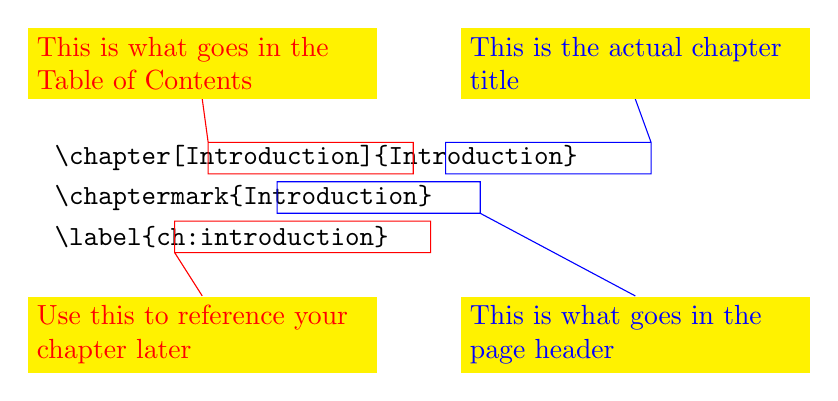
\begin{tikzpicture}
 \draw (0,0) node[anchor=west] {\verb!\chapter[Introduction]{Introduction}!};
 \draw (0,-0.5) node[anchor=west] {\verb!\chaptermark{Introduction}!};
 \draw (0,-1) node[anchor=west] {\verb!\label{ch:introduction}!};

 \draw[color=red]  (4.68,-0.2) rectangle (2.075,0.2) -- (2,0.75) node[anchor=south,fill=yellow,text width=4.2cm] {This is what goes in the Table of Contents};
 \draw[color=blue] (5.09,-0.2) rectangle (7.7,0.2) -- (7.5,0.75) node[anchor=south,fill=yellow,text width=4.2cm] {This is the actual chapter title};
 \draw[color=blue] (2.95,-0.3) rectangle (5.53,-0.7) -- (7.5,-1.75) node[anchor=north,fill=yellow,text width=4.2cm] {This is what goes in the page header};
 \draw[color=red]  (4.9,-0.8) rectangle (1.65,-1.2) -- (2,-1.75) node[anchor=north,fill=yellow,text width=4.2cm] {Use this to reference your chapter later};
\end{tikzpicture}


\subsection{When You Want A New Section}

Same as a new chapter, but use \texttt{\textbackslash section} and \texttt{\textbackslash sectionmark} instead of \texttt{\textbackslash chapter} and \texttt{\textbackslash chaptermark}. Example:
\small\vskip-25pt
\begin{singlespace}
\begin{verbatim}
\section[Table of Contents Name]{Actual Section Name}
\sectionmark{This is what goes in the header}
\label{sec:example}
\end{verbatim}
\end{singlespace}
\normalsize

\subsection{When You Want A New Subsection}

Subsections {\bf should not} change the headers on the page, so there is no command called \st{\texttt{\textbackslash subsectionmark}}. To start a new subsection, use \texttt{\textbackslash subsection} and \texttt{\textbackslash label} (similar usage as \texttt{\textbackslash chapter}). Example:
\small\vskip-25pt
\begin{singlespace}
\begin{verbatim}
\subsection[Table of Contents Name]{Actual Subsection Name}
\label{subsec:example}
\end{verbatim}
\end{singlespace}
\normalsize

\subsection{When You Want A New Subsubsection}

Subsections {\bf should not} change the page header and {\bf should not} appear in the Table of Contents, so there is no command called \st{\texttt{\textbackslash subsubsectionmark}}. To start a new subsubsection, use \texttt{\textbackslash subsubsection} and \texttt{\textbackslash label}. Example:
\small\vskip-25pt
\begin{singlespace}
\begin{verbatim}
\subsubsection{Actual Subsubsection Name}
\label{subsubsec:example}
\end{verbatim}
\end{singlespace}
\normalsize

\section[\texttt{appA.tex}, \texttt{appB.tex}, \dots]{\texttt{appA.tex}, \texttt{appB.tex}, \dots}
\sectionmark{\texttt{appA.tex}, \texttt{appB.tex}, \dots}
\label{sec:app_i_tex}

When you are creating your appendices, you should use the same commands as in Section~\ref{sec:ch_i_tex}. The only difference will be in the output (different numbering style).

\section[\texttt{preamble.tex}]{\texttt{preamble.tex}}
\sectionmark{\texttt{preamble.tex}}
\label{sec:preamble_tex}

In this file, you should place all of your commands that will be used throughout all of your files. To make your code more readable, I recommend placing your \texttt{\textbackslash usepackage} commands in this file. Moreover, any commands which make life easier for you should appear here. Here are a few examples (I recommend that you try each of them, they are very useful when you are writing and editing your thesis).

\begin{lstlisting}
\newcommand{\etal}{\emph{et al.}\xspace}
\newcommand{\CITE}{{\bf {\color{red} [CITE]}}\xspace}
\newcommand{\REF}{{\bf {\color{red} [REF]}}\xspace}
\newcommand{\FIGURE}{{\bf {\color{red} [FIG]}}}
\end{lstlisting}

\section[\texttt{thesis-refs.bib}]{\texttt{thesis-refs.bib}}
\sectionmark{\texttt{thesis-refs.bib}}
\label{sec:thesis_refs_bib}

This is where you can store all of your references. I would recommend using BibTeX since it correctly formats and organizes your references.
